\section{Caso parallelo PRAM - Parallel RAM}
Consiste di un set di processori che hanno una memoria in comune. Questa memoria condivisa fa si che la comunicazione tra i processori sia immediata.

C'è una memoria centrale su cui si affacciano i processori. Questi processori avranno anche la memoria privata perchè per lavorare hanno bisogno anche di registri personali.

La memoria globale è usata dai processori per scambiarsi dati in tempo $O(1)$: perché il processore $k$ e il processore $j$ si scambino un valore, basta che il processore $k$ scriva tale valore in una variabile condivisa e il processore $j$ vi acceda in lettura. Il calcolo procede per passi.

Questo modello di macchine è detto di tipo SIMD (Single Instruction Multiple Data).

\paragraph{Risorse di calcolo} Sono il tempo parallelo richiesto dal nostro algoritmo e il numero di processori, cioè la quantità di hardware messa a disposizione per risolvere il problema
\begin{itemize}
    \item sequenziale: $t(n), s(n)$
    \item parallelo: $p(n), T(n,p(n))$. Dove $n$ è la lunghezza dell'input, $p(n)$ il numero di processori su input di lunghezza $n$ (caso peggiore). E' ovvio che il tempo dipenda non solo dalla lunghezza dell'input ma anche dal numero di processori presi in considerazione.

    $T(n)$ era vero anche nel caso sequenziale, in questo caso diventa anche funzione di $p(n)$, perciò $T(n, p(n))$. Il tempo parallelo dipende anche dal numero di processori utilizzati per l'esecuzione dell'algoritmo

    Quando leggeremo $T(n,1)$ è un caso particolare del tempo parallelo che coincide con il tempo sequenziale. Come caso particolare degli algoritmi paralleli ci sono gli algoritmi sequenziali
\end{itemize}

\paragraph{Valutazione precisa del tempo T(n, p(n))}
Mettiamo la nostra batteria di processori in fila $P_1, P_2, \dots, P(n)$ e metto in colonna le istruzioni eseguite dal processore. \uline{Ogni riga di questa tabella mi dà un passo parallelo}. \uline{Il numero di passi paralleli solitamente dipende dal numero di $n$, l'ultimo passo è $k(n)$}.

\uline{Per ogni passo parallelo prendo il tempo massimo e sommo}. Così ottengo il tempo totale dell'algoritmo. Il tempo del passo i-esimo lo indichiamo così
$$t_i(n) = max\{t_i^j(n)\;|\;1 \leq j \leq p(n)\}$$
E' il massimo tra tutti i tempi dell'i-esimo passo tra tutti i processori $j$.\\
Pertanto il tempo massimo di questo algoritmo non è altro che la somma del tempo richiesto all'i-esimo passo per i che va da 1 a $k(n)$
$$T(n,\;p(n)) = \sum_{i=1}^{k(n)}\;t_i(n)$$
\begin{itemize}
    \item $T$ dipende da $k(n)$
    \item $T$ dipende anche dalla dimensione dell'input $n$
    \item $T$ dipende da $p(n)$
\end{itemize}

Se al posto di $p(n)$ processori ne abbiamo $p(n/2)$, quindi li riduciamo, allora $p1$ esegue le sue istruzioni del primo passo parallelo più le istruzioni che seguono del processore $p(n/2) + 1$. $p2$ eseguirà le sue istruzioni del primo passo parallelo e successivamente le istruzioni di $p(n/2) + 2$ e così via.

\paragraph{Proprietà sulla comunicazione} La comunicazione avviene in tempo costante, infatti se un processore $P_j$ vuole comunicare un dato $x$ a $P_z$ prende dal suo registro personale il dato $x$ e lo scrive in un registro della memoria centrale. $P_z$ sa che è avvenuta questa operazione e va a leggere il dato nella memoria centrale. Questa è la situazione dei multi-core attuali

Con questa struttura siamo in grado di attuare una \uline{forte parallelizzazione, il motivo è dato proprio dalla comunicazione in tempo costante}. Non abbiamo problemi a far comunicare processori anche di indici molto distanti. Non si spreca tempo per la comunicazione, il tempo viene utilizzato tutto per far funzionare i processori sulle istruzioni dell'algoritmo.

\paragraph{Memoria condivisa} La memoria condivisa la chiamiamo \textit{M}, questa memoria condivisa è fatta da una sequenza di registri (per semplicità) che chiamiamo $M[0], M[1], \dots, M[n]$.

Ogni $P_i$ è una RAM sequenziale costituita da una ALU e i suoi registri personali che costituiscono la memoria privata del processore li indicheremo con $R[0], R[1]$. 

\begin{osservazione}
  Quando un'unità di calcolo deve compiere un'operazione (ad esempio una somma) deve avere i dati nella sua memoria privata su particolari registri, dove vengono presi le sequenze di bit e sommati. Anche se parleremo di somma di elementi presi dalla memoria centrale c'è questo passaggio di prendere i dati dai registri $M$ e portarli nei registri privati $R$. Siccome però questa operazione è costante\footnote{Perchè facciamo riferimento al costo uniforme, non logaritmico}, e sempre uguale qualunque sia il dato, faremo somme di numeri in $M$ ma in realtà i dati vengono trasportati da $M$ a $R$  
\end{osservazione}

\paragraph{Istruzioni dei Pi}
Ogni singolo processore nella PRAM, essendo a sua volta una RAM, può effettuare le seguenti operazioni:
\begin{itemize}
    \item Operazioni aritmetico/logiche
    \item Istruzioni da/per la memoria centrale:
    \begin{itemize}
        \item $STORE\;R[K]\;M[h]$, prendi il dato dalla mia memoria privata che sta nel mio registro k-esimo e mettilo nella memoria centrale
        \item $LOAD\;R[K\prime]\;M[h\prime]$, operazione opposta. Prendi il dato che c'è nella memoria centrale nella cella $h\prime$ e portalo nella memoria privata.
    \end{itemize}
\end{itemize}

%Come si programma una PRAM
\begin{comment}
 \paragraph{Come si programma una PRAM?}
L'idea è che c'è un unico programma per tutti i nostri processori, tutti hanno accesso al programma e si caricano le istruzioni una dopo l'altra.   
\end{comment}

\paragraph{Architetture in base alla capacità di accedere alla memoria condivisa}
\begin{enumerate}
    \item \textbf{\textit{EREW}}: no scrittura/lettura stessa cella di $M$. \uline{Non è possibile l'accesso simultaneo alle celle della memoria centrale}. Ad un instante di tempo una cella di memoria può essere letta o scritta da soltanto un processore.
    \item \textbf{\textit{CREW}}: lettura simultanea si, scrittura simultanea no. La scrittura rimane esclusiva
    \item \textbf{\textit{CRCW}}: scrittura/lettura simultanea si. Per la scrittura simultanea abbiamo diverse politiche:
    \begin{itemize}
        \item common, i processori possono scrivere in memoria centrale contemporaneamente solo se vogliono scrivere lo stesso dato pena l'arresto del sistema. Se un processore non è sincronizzato, ha un dato diverso e io faccio l'arresto del sistema.
        \item random, un processore a caso scrive. E' una politica difficile
        \item max/min, si permette al processore $P_i$ solo se ha il dato max o min
        \item priority, scrive il processore $P_i$ con priorità max. I processori non sono tutti uguali ma c'è un certo ordine di importanza. 
    \end{itemize} 
\end{enumerate}

\begin{osservazione}
$\text{EREW} \implies \text{CREW} \implies \text{CRCW}$\\
Non è vero il viceversa, perchè architettura di tipo $2$ e $3$ offrono dei vantaggi rispetto all'architettura di tipo $1$. La \textit{CREW} ha la scrittura simultanea e questo velocizza il nostro algoritmo. L'architettura più ragionevole e semplice a livello hardware è EREW, in questo caso è compito del programmatore disegnare l’algoritmo in modo che non accadano conflitti in lettura o scrittura
\end{osservazione} 

\paragraph{Forma dell'istruzione}
Chiamato anche passo parallelo:
$$for\;all\; i \in I\;par\;do: istruzione_i$$
\textit{par do} cioè fai in parallelo, esegui in parallelo. Si differenzia dal for tradizionale proprio da questo costrutto.

Che cos'è $istruzione_i$?A seconda delle architetture della nostra PRAM abbiamo diverse interpretazioni. Ci sono architetture hardware diverse:
\begin{itemize}
    \item \textit{SIMD}: single instruction multiple data.\\
    L'istruzione è uguale per tutti i processori però avviene su dati diversi, su diversi registri.
    \item \textit{MIMD}: multiple instruction multiple data\\
    Abbiamo la possibilità per processori diversi di eseguire istruzioni differenti
\end{itemize}

%Sintesi

\paragraph{Valutazione}
Cos'è efficiente nel caso parallelo? Nel caso sequenziale è \textit{P}, problemi risolti in tempo polinomiale, nel caso parallelo deve essere meglio del tempo polinomiale.

Definiremo un parametro \textbf{\textit{E}: efficienza}, che tiene conto sia del tempo impiegato dal nostro algoritmo che del numero di processori. Se devo avere un'esplosione esponenziale dei processori non conviene. Quindi il tempo deve essere migliore e i processori devono essere contenuti, altrimenti non conviene. Il parametro efficienza ci deve dire se la nostra soluzione parallela è preferibile ad una efficiente soluzione sequenziale

Valuteremo la nostra funzione di tempo $T(n, p(n))$ con il tempo richiesto dall'algoritmo sequenziale $T(n, 1)$. \uline{Se la nostra funzione ha un tasso di crescita inferiore rispetto a quella sequenziale vuol dire che abbiamo migliorato la nostra soluzione}. 
Abbiamo due casi
\begin{itemize}
    \item $T(n,p(n)) = \Theta (T(n,1))$, uguale al tempo sequenziale. Vuol dire che è limitato superiormente e inferiormente dalla funzione sequenziale $T(n,1)$. Il tasso di crescita del tempo parallelo è circa uguale, asintotica alla funzione $T(n,1)$ di tipo sequenziale. E' il caso che noi vogliamo evitare
    \item $T(n,p(n)) = o(T(n,1))$. Vuol dire che cresce più lentamente rispetto al tempo sequenziale. Se faccio il rapporto tra tempo sequenziale e tempo parallelo ho qualcosa che tende ad infinito. E' il caso che vogliamo
\end{itemize}

\paragraph{Speed-up} 
$$S(n, p(n)) = \frac{T(n, 1)}{T(n, p(n))}$$
Esempio: $S=4$ l'algoritmo parallelo è $4$ volte più veloce del sequenziale, ma ricadremo nel primo caso. Quello che vogliamo è che lo \textit{speed-up} sia infinito perchè così abbiamo il secondo caso.
$$S(n,p(n)) \rightarrow \infty$$
Questo non ci dice niente rispetto al valore della risorsa $p(n)$, magari abbiamo utilizzato un numero di processori esagerato. \uline{Non riusciamo a considerare il numero dei processori}. Questo parametro perciò viene utilizzato solo per definire successivamente il parametro efficienza.

\paragraph{Efficienza}
$$E(n,p(n)) = \frac{S(n,p(n))}{p(n)} = \frac{T(n,1)*}{p(n)T(n,p(n))}$$
* si intende il tempo del miglior algoritmo sequenziale. Andiamo a scegliere la funzione tempo più piccola possibile.

Se $E \rightarrow 0$ non va bene, infatti dato che $T(n,p(n)) = o(T,(n,1))$ deve essere che $p(n)$ cresce troppo velocemente. 

Perchè se tende a $0$ stiamo usando troppi processori? Quando lo \textit{speed-up} tende ad infinito vuol dire che i tempi vanno bene, cioè il parallelo è un o piccolo del sequenziale. Se il tempo parallelo non abbatte il tempo sequenziale devono essere i processori che abbattono il tempo sequenziale e quindi stiamo utilizzando troppi processori.

$$0 \leq E(n, p(n)) \leq 1$$

Che sia positivo si vede dalla formula. Che invece il parametro \textit{E} non supera il valore $1$ è da dimostrare.

%Se E->0 stiamo usando troppo hw
\begin{comment}
Esempio: soddisficibilità di formule
$$E(n,p(n)) = \frac{2^n}{2^n\;n} = \frac{1}{n} \rightarrow 0$$
Quando $E \rightarrow 0$ il nostro algoritmo non è così buono perchè ha un costo hardware toppo alto. Stiamo utilizzando troppi processori.
\end{comment}

\begin{dimostrazione}
\textbf{Attraverso algoritmo parallelo $\rightarrow$ algoritmo sequenziale}

Come possiamo ottenere un algoritmo sequenziale se noi abbiamo un algoritmo parallelo? Sostituiamo a $p(n)$ processori un processore solo e mandiamo in esecuzione tutte le istruzioni del primo passo, poi del secondo, etc. Ora vogliamo valutare il tempo di esecuzione dell'algoritmo sequenziale che otteniamo. 

Chiamo $\Tilde{T}(n,1)$ il tempo richiesto dall'algoritmo sequenziale che ho appena descritto, ottenuto direttamente dall'algoritmo parallelo.
Otteniamo un particolare algoritmo sequenziale e il tempo è sicuramente peggiore del miglior algoritmo sequenziale $T(n,1) \leq \Tilde{T}(n,1)$

Il tempo massimo del primo passo parallelo è $t_1(n)\;\text{,}\;p(n) * t_1(n)$ perchè devo fare $p(n)$ mini-programmi, perciò
$$T(n,1) \leq \Tilde{T(n,1)} \leq pn\;t_1(n) + pn\;t_2(n) \dots p(n)\;t_{k(n)}(n)$$

Ora posso raccogliere a fattor comune $p(n)$ e ottengo $p(n)\;\sum_{i=1}^{k(n)}\;t_i(n)$ dove $t_i(n)$ è il tempo di ogni singolo passo parallelo. Ma quest'ultima parte non è nient altro che il tempo parallelo $p(n)T(n,p(n))$

Quindi abbiamo che il miglior tempo sequenziale $T(n,1)$ è limitato superiormente da $p(n)T(n,p(n))$ cioè $p(n)$ per il tempo parallelo. Si ottiene 
$$T(n,1) \leq p(n)\;T(n,p(n))$$
Cosa succede se dividiamo entrambo i lati di questa disuguaglianza per $p(n)$?

$$\frac{T(n,1)}{p(n)} \leq T(n,p(n))$$

Otteniamo che \uline{il nostro tempo parallelo ha un lower bound}, ha un limite inferiore, e questo limite è dato dal rapporto tra il miglior tempo sequenziale diviso il numero di processori. Cioè la cosa migliore che io posso fare è prendere il miglior algoritmo sequenziale ed equi-distribuire le istruzioni tra tutti i processori che lavorano per parallelizzare l'algoritmo.

Ora dividiamo anche per il tempo parallelo $T(n,p(n))$, significa portarlo a sinistra della disuguaglianza, otteniamo a sinistra il parametro efficienza e a destra otteniamo $1$

$$\frac{T(n,1)}{p(n)T(n,p(n))} \leq 1 \equiv E(n,p(n)) = 1$$

Abbiamo dimostrato che l'efficienza non può essere più grande di $1$.
Il meglio che posso avere è $E \rightarrow K \leq 1$ dove $K$ è una costante limitata da $1$ superiormente
\end{dimostrazione}

\begin{dimostrazione} Principio di Wyllie

    \textit{"Se $E \rightarrow 0$ allora per migliorare l'algoritmo provo a ridurre $p(n)$ senza degradare il tempo"}

    Studiare il parametro efficienza facendo crescere/diminuire il numero di processori, cambiando il numero di processori nella formula.

    In particolare è stata data la ricetta di J.Wyllie nella sua tesi del PhD che dice la seguente cosa:
    Se noi diamo un algoritmo parallelo, calcoliamo il parametro efficienza e questo tende a $0$ allora non necessariamente va buttato l'intero algoritmo ma forse si può fare qualcosa per migliorare il parametro efficienza e quindi ottenere un algoritmo buono. Si può migliorare provando a ridurre il numero di processori senza però degradare troppo il tempo (non devo avere un tempo che cambia il tasso di crescita).

    Vediamo la validità di questo principio cambiando il numero di processori da $p\; \text{a}\; \frac{p}{k}$. Raggruppo $p$ lavori a $k$, quindi \uline{un processore anzichè trovarsi $1$ programma se ne trova $k$ e li deve eseguire in sequenza}. Quanto tempo richiede per eseguire $k$ lavori? Il tempo di ogni programmino è limitato superiormente da $k\;t_i(n)$ perchè $t_i(n)$ è il massimo tempo richiesto tra tutti i programmini all'i-esimo passo e non può essere superiore a $k\;t_i(n)$ perchè ne esegue $k$ che vengono eseguiti in sequenza.

    Il tempo parallelo richiesto dal nostro algoritmo fatto in questo modo è limitato superiormente dalla somma dell'i-esimo passo parallelo. Ma l'i-esimo passo parallelo è limitato da $kt_i(n)$. Otteniamo
    $$T(n, \frac{p}{k}) \leq \sum_{i=1}^{k(n)} k\;t_i(n) = k T(n,p)$$

    Questo $k$ è in comune ad ogni elemento della sommatoria perciò posso raccogliere $k$ fuori dalla sommatoria e ottengo

    $$T(n,\frac{p}{k}) \leq k\;T(n, p)$$
    
    Il tempo dell'algoritmo che utilizza $\frac{p}{k}$ processori anzichè $p$ processori è limitato superiormente da $k$ volte il tempo richiesto dall'algoritmo che utilizza $p$ processori.

    Partendo da questa disuguaglianza quello che si ottiene è che \uline{il parametro E cresce col diminuire dei processori}. Questo è vero tenendo la funzione tempo parallelo fissata, cioè senza far degradare troppo il tempo. Quanto vale $E(n, \frac{p}{k})$?
    $$E(n,\frac{p}{k}) = \frac{T(n,1)}{\frac{p}{k}\;T(n,\frac{p}{k})} \geq \frac{T(n,1)}{\frac{p}{k}\;kT(n,p)} = E(n,p)$$

    La formula mostra che diminuendo i processori migliora il parametro efficienza (ciò rende vera la ricetta di Wyllie). \uline{In sostanza ottengo il rapporto tra tempo sequenziale e tempo parallelo su $p$ processori (dopo le semplificazioni), questo per definizione non è nient'altro che l'efficienza su $p$ processori}. \uline{Quindi diminuendo il numero di processori da $p$ a $\frac{p}{k}$ l'efficienza migliora}.

    Vediamo se $k$, nella formula di prima, lo facciamo tendere a $p$ in modo da voler verificare cosa succede se diminuisco il numero di processori aumentando $k$. Sempre meno processori arrivando all'estremo fino ad arrivare ad avere $\frac{p}{p}$

    $$1=E(n,1)=E(n,\frac{p}{p}) \geq E(n,\frac{p}{k}) \geq E(n,p)$$

    (A destra) se confronto l'algoritmo con $\frac{p}{k}$ e quello con $p$ il primo mi da un efficienza migliore. (A sinistra) ho diminuito i processori ($\frac{p}{p}$) e quindi l'efficienza migliora, ecco perchè ho un $\geq$. Però questa non è altro che l'efficienza calcolata con un processore $E(n,1)$ che è sostanzialmente il tempo sequenziale (perchè avrò tempo sequenziale su tempo sequenziale, cioè $1$).

    In questo modo abbiamo ottenuto che l'efficienza di un algoritmo parallelo che usa $p$ processori è limitata superiormente da $1$.
\end{dimostrazione}

\newpage


\subsection{Sommatoria}
Utilizziamo più processori, ogni processore si prende una somma e poi una volta ottenuti gli esiti parziali dobbiamo fonderli per ottenere il risultato della sommatoria

Input: $M[1], M[2], \dots , M[n]$\\
Output: $M[n] = \sum_{i=1}^n M[i]$

Supponiamo che i valori $n$ siano nella memoria centrale, quindi nelle celle $M[1], M[2], \dots , M[n]$. Il risultato lo scriveremo nell'ultima cella $M[n]$.

\paragraph{Algoritmo sequenziale}
Il migliore algoritmo sequenziale è dato da questo codice
\begin{lstlisting}
    for i=1 to n-1 do
        M[n] = M[n] + M[i]
\end{lstlisting}
Siccome vogliamo il risultato in $M[n]$ questo algoritmo somma tutto in $M[n]$ utilizzandolo come un accumulatore, escludendo chiaramente $n$ perchè viene sommato alla prima iterazione. Quante istruzioni sono? $n-1$ per cui il tempo di questo algoritmo sequenziale è proprio $T(n,1) = n-1$ e non posso scendere al di sotto di questo valore perchè le somme devo farle tutte.

\paragraph{Idea per parallelizzare} "Una somma a processore", ma in questo modo non stiamo dicendo quale somma

\begin{figure}[h]
    \centering
    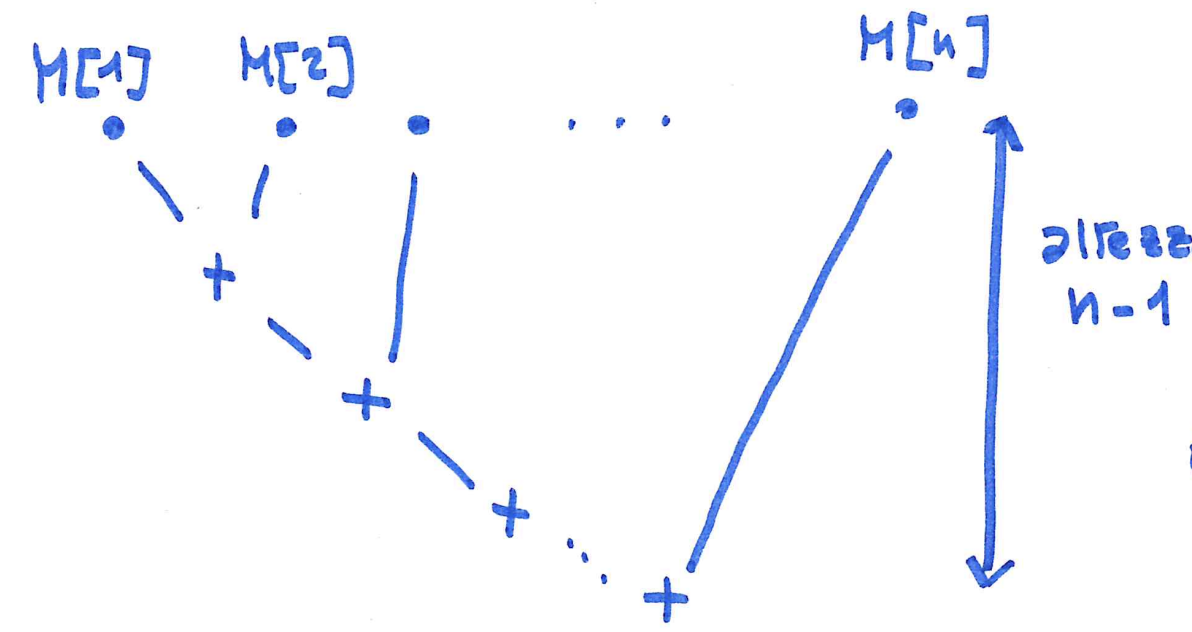
\includegraphics[scale=0.4]{images/idea_sommatoria.png}
\end{figure}

Rappresentiamo il nostro algoritmo come un albero (sbilanciato) che ha come foglie i dati di input, le celle $M[1], M[2], M[n]$, e i livelli dell'albero rappresentano i passi paralleli del nostro algoritmo. Ogni livello di quest'albero è un passo parallelo e mi vengono fuori $n-1$ passi. Qual'è l'efficienza di questo algoritmo?

$$E=\frac{n-1}{(n-1)(n-1)} \rightarrow 0$$

Il tempo sequenziale sopra che abbiamo calcolato dall'algoritmo sequenziale. Ogni processore fa una somma perciò avrò $n-1$ somme quindi $n-1$ processori per il tempo dell'algoritmo parallelo che è $n-1$. Tende a $0$ quindi non è efficiente. Se il tempo è uguale al sequenziale non ho parallelizzato niente, non ha senso calcolare il parametro efficienza. \uline{L'altezza risulta essere il tempo dell'algoritmo}.

\paragraph{Alternativa} Posso fare qualcosa di diverso perchè la somma è associativa\footnote{$((a+b)+c)+d = (a+b) + (c+d)$}, non conta l'ordine con cui facciamo le somme. In più da un albero \textit{sbilanciato} mi muovo su un albero \textit{bilanciato}

\begin{figure}[h]
    \centering
    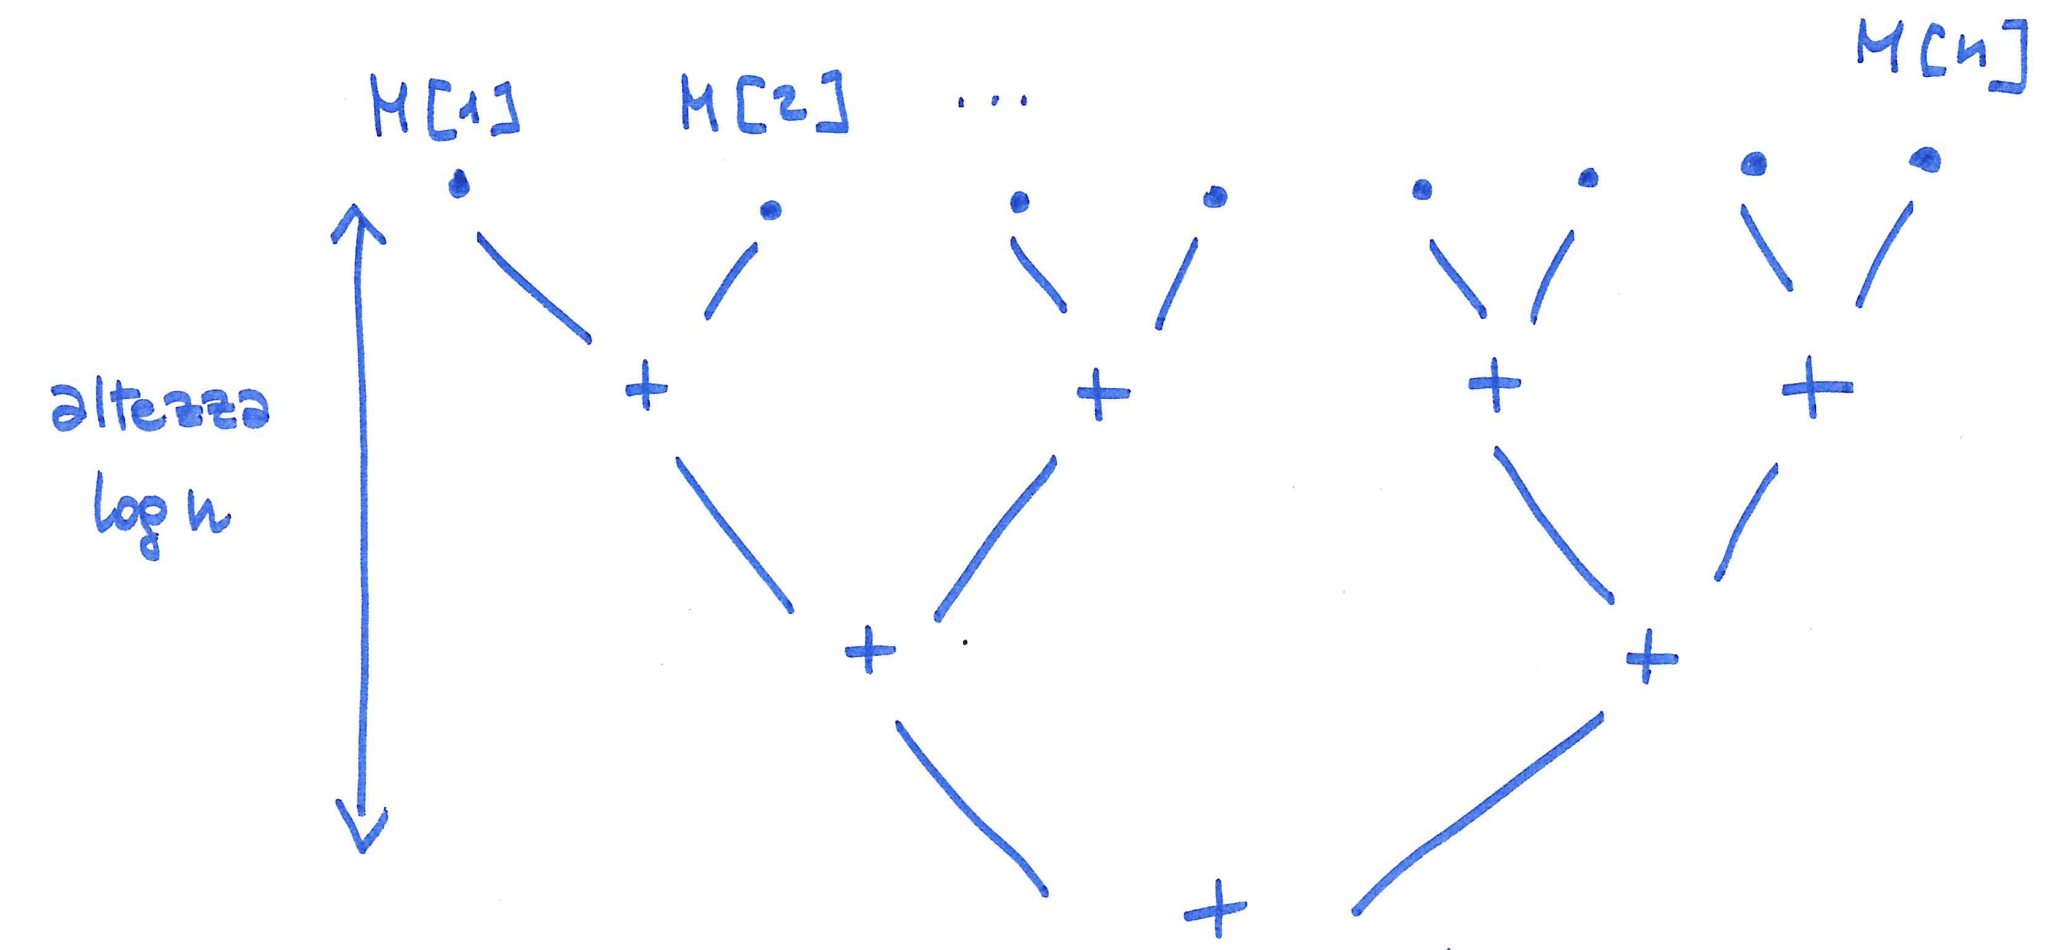
\includegraphics[scale=0.35]{images/idea2_sommatoria.png}
    \caption{Alternativa per parallelizzare}
\end{figure}

\uline{Stiamo assumendo che $n$ è potenza di $2$}. Cosa manca in questo schema? Non abbiamo detto come fanno i processori a comunicarsi gli esiti. L'idea è che li vanno a \uline{sovra-scrivere nelle celle di memoria dell'input}.

\paragraph{Algoritmo EREW}
In questo caso le celle sono lette e scritte in maniera esclusiva, non ci sono letture e scritture simultanee. In una PRAM serve sapere anche dove andiamo a memorizzare gli esiti parziali perchè tutti i processori devono essere d'accordo sulla cella condivisa che contiene il risultato.

\begin{figure}[h]
    \centering
    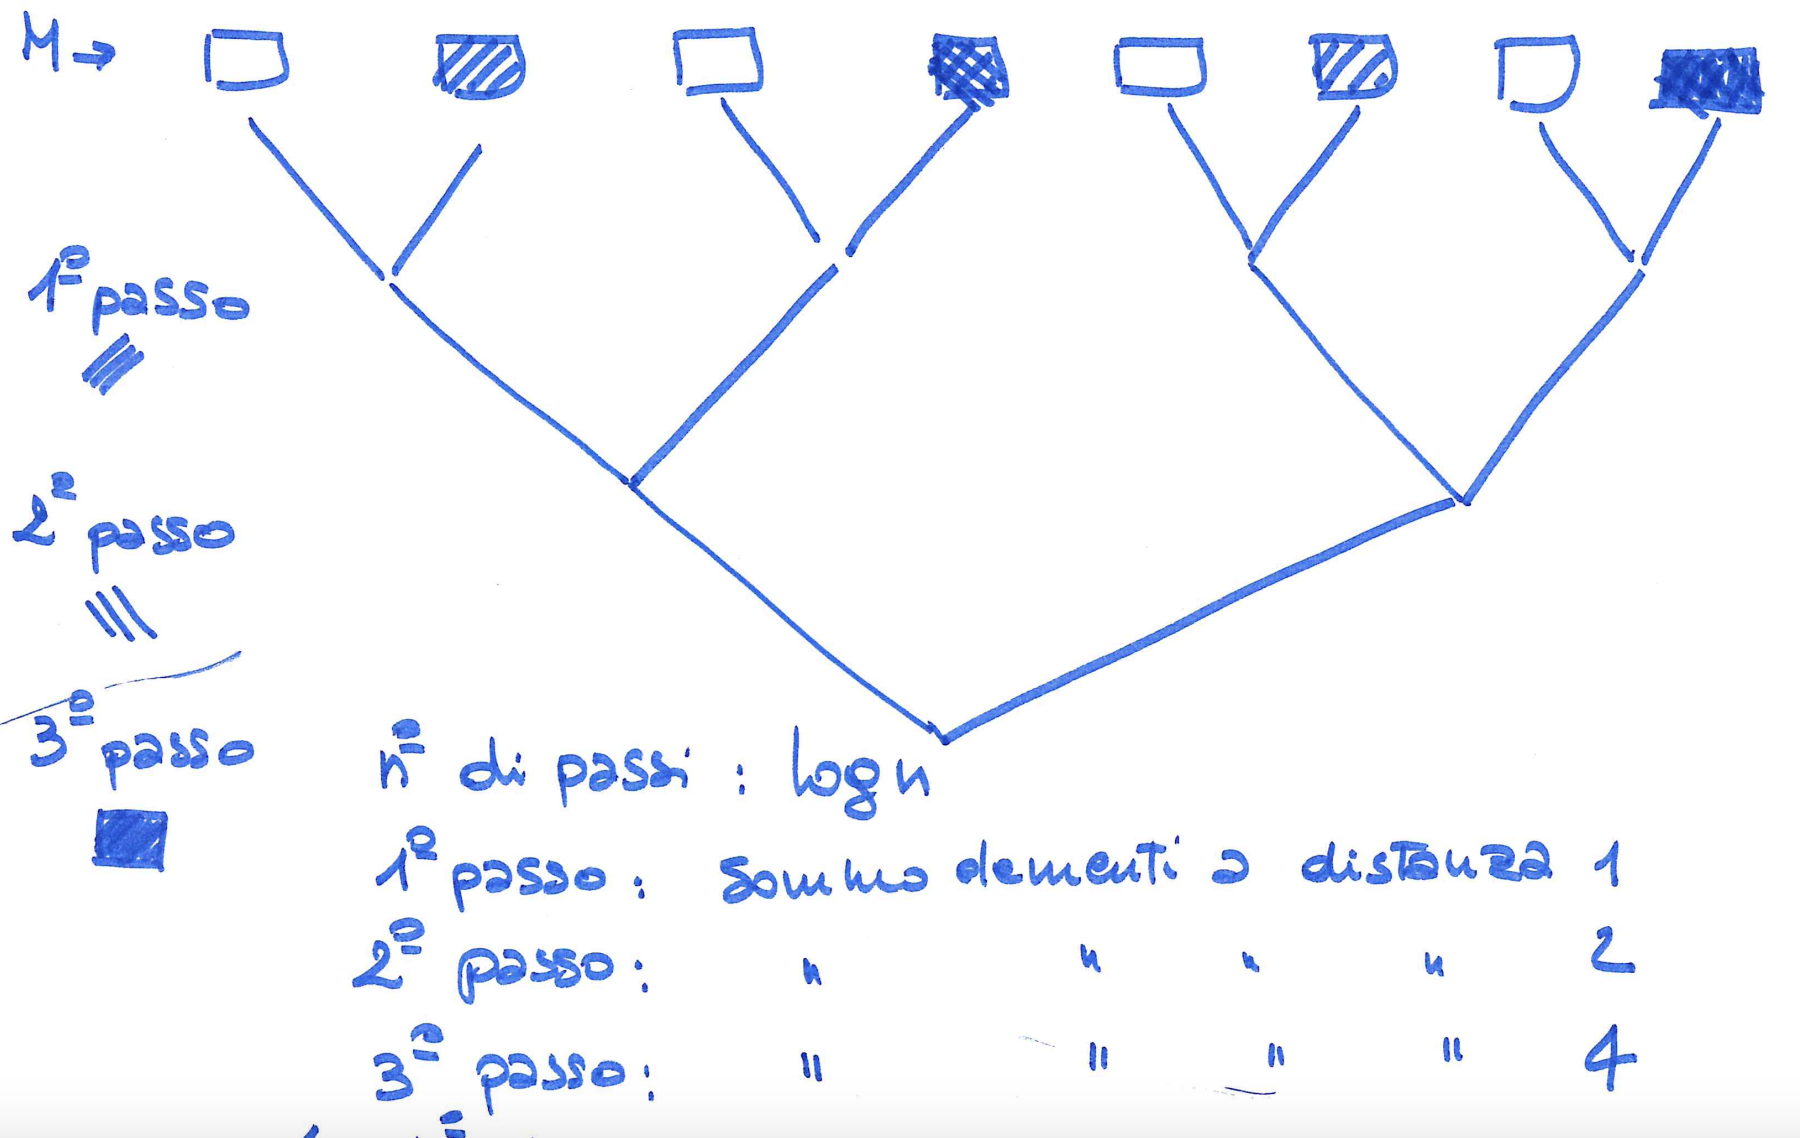
\includegraphics[scale=0.4]{images/erew_sommatoria.png}
    \caption{Algoritmo EREW sommatoria}
\end{figure}

\uline{Il risultato si pone nella cella con indice più alto}. Al primo passo si somma l'indice dispari con quello pari. Al secondo passo i processori sanno che i dati su cui calcolare la somma sono quelli di indice pari. La distanza è una potenza di $2$ e aumenta man mano che aumenta l'indice del passo parallelo. Il numero di passi di questo algoritmo risulta essere $\log n$ perchè abbiamo un albero completamente bilanciato

Istruzioni:
Consideriamo \textit{k} come gli indici dei processori e i passi sono paralleli
\begin{enumerate}
    \item passo: $M[2k] = M[2k] + M[2k-1]$ con $1 \leq k \leq \frac{n}{2}$
    \item passo: $M[4k] = M[4k] + M[4k-2]$ con $1 \leq k \leq \frac{n}{4}$
    \item passo: $M[8k] = M[8k] + M[8k-4]$ con $1 \leq k \leq \frac{n}{8}$
    \item $\dots$
    \item $\log n$ passo: $M[n] = M[n] + M[\frac{n}{2}]$ 
\end{enumerate}

\paragraph{Pseudo-codice} Dove $j$ è l'indice del passo parallelo
\begin{minted}
    [
    frame=lines,
    framesep=2mm,
    baselinestretch=1.2,
    bgcolor=white,
    fontsize=\footnotesize,
    linenos
    ]{python}
    for j in range(1, logn):
        for k in range(1, n // 2**j + 1):
            M[2**j*k] = M[2**j*k] + M[2**j*k - 2**(j-1)]
    return M[n]
\end{minted}
Il primo ciclo for scandisce i passi paralleli (l'indice dei passi paralleli è j), il secondo è un for par do quindi è un passo parallelo e fa lavorare $\frac{n}{2^j}$ processori al passo $j$ 

\paragraph{Dimostrazione EREW}
E' \textit{EREW}? Solo il processore \textit{k} può leggere e fare operazioni, gli altri utilizzano altre celle.

Come due processori $a$ e $b$ che lavorano nello stesso passo parallelo le celle che vanno a toccare risultano essere diverse tra di loro.

\begin{dimostrazione}
Dobbiamo dimostrare che al j-esimo passo vale questa proprietà
$$M[2^jk]=M[2^jk]+ \dots + M[2^j(k-1)+1]$$
Dove $j$ è un qualcosa compreso tra $[1, \log n]$, l'indice del passo parallelo. Dobbiamo dimostrare che nelle celle multiple di $2^j$ ci sono $2^j$ valori sommati di tutte le $2^j$ celle precedenti  

La dimostrazione è una dimostrazione per induzione su j. Andiamo a sostituire nella star (prima equazione) $\log n$ al posto di $j$. Inoltre siccome siamo al passo $\log n$ sappiamo che viene utilizzato un solo processore che è quello che fa la somma dei due risultati parziali che lavorano sulla metà dell'input. Allora $k=1$ perchè c'è un solo processore. In questo caso la proprietà è
$$M[n] = M[n] + \dots + M[1]$$
Mi viene che in $M[n]$ ci va la somma di tutti i precedenti valori. Se è vera questa proprietà, questo dimostra che il mio algoritmo è corretto.

CASO BASE: $j=1$ e $1 \leq k \leq \frac{n}{2}$\\
Istruzione dell'algoritmo $\rightarrow M[2K] = M[2K] + M[2K-1]$ quindi vale la proprietà star 

PASSO INDUTTIVO: Supponiamo vera la proprietà star per l'indice $j-1$ e dimostriamo che la manteniamo anche per il passo successivo, dimostriamo che vale anche per $j$
\end{dimostrazione}

\subsubsection{Valutazione dell'algoritmo sommatoria}

\paragraph{Numero di processori}
Il numero di processori $p(n) = \frac{n}{2}$. Il livello più costoso in termini di processori è il primo, quindi prendo quello. E' vero che al passo successivo la metà di questi sono inutilizzati, ciò potrebbe suggerirci che stiamo usando troppi processori

\paragraph{Tempo}
Abbiamo detto che l'altezza dell'albero è $\log n$ perciò il tempo deve essere logaritmico, andiamo a considerare le micro-istruzioni: LD, LD, ADD, ST. $4$ micro-istruzioni, perciò il tempo parallelo calcolato su $T(n, \frac{n}{2}) = 4 \log n$

\begin{osservazione}
    Un piccolo accorgimento dobbiamo farlo se $n$ non è potenza di $2$. Abbiamo detto che lavora bene su $n$ potenza di $2$ perchè ci da un albero bilanciato. Idea: allunghiamo l'input di $0$ fino alla potenza di $2$ successiva ad \textit{n}. Cioè da \textit{n} binario a $2n$. Va bene mettere lo $0$ perchè non modifica il risultato totale. 

    La potenza più vicina ad \textit{n} la posso trovare in binario. Cioè da \textit{n} in binario la successiva potenza di due ha un bit in più impostato ad $1$ e poi $0$, cioè $1 0 0 \dots 0$. Questa distanza di $2$ la troviamo tra \textit{n} e $2n$, infatti se scriviamo $2n$ in binario è \textit{n} in binario a cui abbiamo aggiunto uno $0$ finale.

    Pertanto avrò:\\
    $p(n) = \frac{2n}{2} = n$ ; 
    $T(n,n) = 4 \log 2n \leq 5 \log n$ ;\\
    $\implies p(n) = O(n)$ e $T(n,n) = O(\log n)$

    Se non vogliamo considerare le costanti possiamo dire che abbiamo un algoritmo parallelo il quale ha numero di processori lineare $O(n)$ e tempo parallelo $O(\log n)$

    \paragraph{Efficienza}
    $E(n,n) = \frac{n-1}{n\;5\log n} \approx \frac{N}{5 \log n} \rightarrow 0$ lentamente
    
    Sopra il tempo sequenziale. Sotto abbiamo il numero di processori che è $n$ per $\log n$ che è il tempo parallelo, si  semplifica $n$ rimane $\frac{1}{\log n}$ che tende a $0$, lentamente ma tende a $0$
\end{osservazione}

\paragraph{Principio di Wyllie}
Visto che i processori sono un pò sprecati applicchiamo Wyllie, vediamo se riusciamo a diminuire il numero di processori e cerchiamo di mantenere lo stesso tempo per avere $p(n) = o(n) \wedge E \rightarrow C \neq 0$

Invece di avere $\frac{n}{2}$ ci sono solo p processori e andiamo a vedere che valore ci va bene. Questi processori non dovranno prendersi solo due valori in carico ma un po di più perchè $p < \frac{n}{2}$. Supponiamo che il numero di dati che si prende in carico ogni singolo processore sia un valore $\Delta$, cioè sto raggruppando n numeri in p gruppi. $\Delta = \frac{n}{p}$

Abbiamo scoperto che un \textit{p} ragionevole c'è ed è $\frac{n}{\log n}$, allora con un numero di processori $p = \frac{n}{\log n}$ otteniamo un'efficienza costante $\neq 0$. Quindi se noi raggruppiamo i nostri $n$ lavori in gruppi di cardinalità $\log n$ raggiungiamo il nostro scopo. Il numero di processori che prima era $n$ diventa $\frac{n}{\log n}$ e il tempo rimane comunque parallelo perchè il primo passo che consiste nella sequenzializzazione dei $\log n$ lavori che sono stati raggruppati e affidati ai $p$ processori consiste di un tempo che è $\log n$.

 Il primo passo parallelo che è la sequenzializzazione di $\log n$ somme, costa $\log n$. E' un passo parallelo ma questi numeri vengono sommati in sequenza dai miei $p$ processori. Otteniamo nelle celle $> \Delta$ la somma dei $\log n$ numeri precedenti e applicando a queste celle l'algoritmo sommatoria otteniamo il nostro algoritmo efficiente.

\paragraph{Riassumendo}
Abbiamo un numero di processori che è $p(n) = \frac{n}{\log n}$ e tempo parallelo. La prima fase è la sequenzializzaione dei $\log n$ numeri e quindi costa $\log n$. La seconda fase consiste nell'applicare l'algoritmo sommatoria alle celle multiple di $\Delta$.
L'efficienza è stata calcolata
$$E \approx \frac{n-1}{2n} = \frac{1}{2}$$

\paragraph{Lower bound idea} Ogni algoritmo parallelo che si può immaginare per questo problema viene visualizzato da un albero binario perchè la somma è un'operazione binaria. Quindi può essere descritto da un albero binario ma siccome le foglie sono i dati di input il numero di foglie di quest'albero binario è $n$ e il tempo dell'algoritmo parallelo risulta essere l'altezza dell'albero

Ora c'è una relazione tra $n$ e l'altezza dell'albero che è la seguente: 
$$n = \#\;di\;foglie\; \leq 2^h \implies h \geq \log n$$
Il numero di foglie è limitato superiormente da $2^h$ dove h è l'altezza dell'albero, da cui ricavo che se ho $n$ come numero di foglie, l'altezza deve essere almeno $\log n$.

Abbiamo detto che l'altezza dell'albero è il tempo dell'algoritmo parallelo. Quindi un algoritmo parallelo che risolve il problema sommatoria deve essere almeno logaritmico, lo abbiamo trovato.


\subsection{Somme prefisse}
Data una sommatoria, individuare i risultati parziali dei prefissi delle somme della sommatoria. Esempio: la sommatoria consiste di $3$ numeri: $2+4+6$, le somme prefisse sono i prefissi della sequenza $2, 4, 6$ quindi la somma di $2$, poi $2+4$ e poi $2+4+6$.

Anche il problema delle somme prefisse contiene al suo interno il problema della sommatoria, però questa volta viene risolta in maniera completamente diversa.

Input: $M[1], M[2], \dots , M[n]$\\
Output: $\sum_{i=1}^k\;M[i] \rightarrow M[k]\;\;\; 1\leq k\leq n$

Alla cella $M[k]$ ci deve essere la somma di tutti i numeri precedenti, compreso $M[k]$. Sostanzialmente su qualunque posizione all'interno di questa sequenza io mi fermo ed individuo un prefisso. Se mi fermo su $M[2]$, avrò prefisso $M[1], M[2]$. Il problema delle somme prefisse consiste nel calcolare la somma di tutti i prefissi della sequenza e di andare  a posizionare il risultato nella cella di indice maggiore.

\paragraph{Algoritmo sequenziale}
Il vettore M di elementi da $M[1]$ ad $M[n]$.
Le operazioni vengono eseguite in sequenza, vengono risolte le frecce in sequenza. Prima operazione prendere $M[1]$ sommarlo ad $M[2]$ e lo si mette nella cella $M[2]$. Al secondo passo si prende il valore di $M[2]$ e si mette nella cella $M[3]$, a questo punto quest'ultima conterrà il valore di $M1, M2, M3$. 

\begin{lstlisting}
    for k=2 to n do
        M[k] = M[k] + M[k-1];
\end{lstlisting}

Il tempo è $n-1$, abbiamo $n-1$ frecce quindi avrò $n-1$ passi.

\paragraph{Una proposta parallela per somme prefisse} Ho un array che mi rappresenta i dati di input, quindi le celle M della memoria centrale.

Ho già osservato che l'ultimo elemento è la somma di tutti, allora io prendo il modulo sommatoria gli do in input tutti i valori da $M[1]$ ad $M[n]$ e applico il modulo sommatoria, il risultato lo metterò nella cella con indice più alto, quindi $M[n]$. \uline{Risolvo con sommatoria tutti i possibili prefissi}. Si applicano $n-1$ moduli sommatoria.

Questo non è un algoritmo EREW, perchè il dato in input viene passato a tutti i moduli sommatoria. C'è una condivisione degli input, accedono simultaneamente ad una cella.

Però è un algoritmo CREW su PRAM. I moduli che utilizziamo nell'algoritmo sono $n-1$,  ogni modulo risolve il problema sommatoria e il problema sommatoria si risolve con $\frac{n}{\log n}$ processori.

Perciò numero di processori
$$ p(n) \leq (n-1)\frac{n}{\log n} \approx \frac{n^2}{\log n} = \sum_{i=2}^n \frac{i}{\log i} \geq \frac{1}{\log n} \sum_{i=2}^n i \approx \frac{n^2}{\log n}$$

$\log n$ per il modulo che prende in input $n$, per un modulo che prende lunghezza $i$ avremo $\log i$. Il tempo di ogni modulo sommatoria è $\log n$ perchè ogni modulo è profondo $\log n$
$$T(n,p(n)) \approx \log n $$

\paragraph{Efficienza}
$$E \approx \frac{n-1}{\frac{n^2}{\log n} \log n} \rightarrow 0$$
Poco efficiente

\subsubsection{Pointer doubling di Kogge-Stone}
Un algoritmo migliore è dato da \textit{Kogge-Stone} nel $'73$ utilizzando i pointer doubling: sono dei puntatori (dei link) tra coppie di numeri, indicati con una freccia,che risolve il problema delle somme prefisse. \uline{Si stabiliscono dei legami tra i numeri}. \uline{Ogni processore si occupa di un legame e ne fa la somma}

\begin{center}
    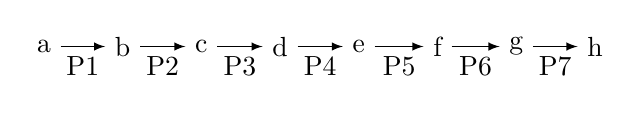
\begin{tikzpicture}[>=latex]
      % Nodes
      \foreach \i/\label in {1/a, 2/b, 3/c, 4/d, 5/e, 6/f, 7/g, 8/h}
        \node (P\i) at (\i,0) {\label};
    
      % Arrows and Labels
      \foreach \i in {1,...,7}
        \draw[->] (P\i) -- node[below] {P\i} (P\the\numexpr\i+1\relax);
    
    \end{tikzpicture}
\end{center}

Per ogni freccia c'è un processore, ne fa la somma e lo mette nella cella con indice più alto. Vengono aggiornati i link al passo $J=1$, dopo aver fatto le somme parziali. Quando $J=1$ il link è tra un elemento e il suo successore, a distanza $1$. Inizialmente in memoria centrale/condivisa si troveranno gli $8$ elementi $M[i]$ o $M[K]$ del nostro input più si troverà anche un vettore $S$ che è il vettore dei link che dice di un elemento qual'è il suo successore. All'inizio se l'elemento è $K$ allora $S[K]=K+1$. Per ogni link/puntatore dedico un processore, e il processore prende l'elemento di indice più basso, lo somma e lo posiziona nell'elemento con indice più alto

\uline{Queste frecce vengono raddoppiate, ecco perchè \textit{pointer doubling}}. Al posto di andare dal proprio elemento al successivo viene messo un link a distanza $2$.

Gli ultimi due elementi non hanno successori, in questo caso \textit{g} e \textit{h}, perchè non ci sono abbastanza elementi per assegnargli un successore. Man mano che iteriamo il passo parallelo il numero di elementi che non ha successore aumenta, cioè raddoppia.

Al passo $J=2$ vengono raddoppiati nuovamente i link, invece che distanza $2$ si va a distanza $4$

Il numero di elementi che non hanno successori è aumentato, al passo $J=1$ ne avevamo $2$, al passo $J=2$ ne abbiamo $4$. Al passo $J=3$ i puntatori non possono essere più assegnati, questo decreta la fine dell'algoritmo.

\begin{enumerate}
    \item Quanti numeri privi di successore genera il j-esimo passo?\\
    Il passo $J=1$ ne genera $2$, il passo $J=2$ quando aggiorna ne genera $4$, quindi $2^J$. Il numero di passi dell'algoritmo è logaritmico, ad ogni passo $J$ gli elementi privi di successore sono $2^J$
    \item Quanti passi dura l'algoritmo? L'algoritmo dura fintanto che ho successori.
    \item Quali processori attivo al j-esimo passo?
    $$1 \leq K \leq n-2^{j-1}$$
    Ad ogni passo diminuisce il numero di successori, quindi di link. Partiamo dal numero di processori che è $n-1$ ed arriviamo a $\frac{n}{2}$
    \item Sia $S[K]$ la posizione del successivo di $M[K]$ come inizializzo S?
    $$S[K]=K+1\;\;,\; S[n]=0$$
    Il vettore S è il vettore dei successori.
    \item Dato $P_k$, quale istruzione su M deve eseguire? $$M[K]+M[S[K]] \rightarrow M[S[K]]$$
    Risolvere un link comporta la somma di due elementi. Dopo aver fatto la somma si fa l'aggiornamento dell'array S. Come?
    \begin{lstlisting}
        S[K] = (S[K]==0? 0 : S[S[K]])
    \end{lstlisting}
    Nullo se non aveva successori, altrimenti va raddoppiato (con $S[S[K]]$). In questo caso devo raddoppiare la freccia, cioè dovrà puntare al successore del successore di K
\end{enumerate}

\paragraph{Codice dell'algoritmo parallelo}:
\begin{minted}
    [
    frame=lines,
    framesep=2mm,
    baselinestretch=1.2,
    bgcolor=white,
    fontsize=\footnotesize,
    linenos
    ]{python}
    for j in range(1, logn):
    for k in range(1, n // 2**j + 1):
    M[S[k]] = M[k] + M[S[k]]
    S[k] = 0 if S[k] == 0 else S[S[k]]
\end{minted}

 La cosa intelligente è che in realtà benchè $K$ e $K\prime$ utilizzano la stessa cella di memoria lo fanno in tempi diversi.

\paragraph{Correttezza}
\begin{enumerate}
    \item E' \textit{ EREW P-RAM}\\
    $P_k$ lavora su $M[K]$ e $M[S[K]]$:\\
    se $i \neq j \implies S[i] \neq S[j]$, quindi hanno successori diversi

    Osserviamo infine che, durante l’esecuzione, il vettore S è tale che, se $i\neq j, S(i)\neq 0, S(j) \neq 0, \text{allora}\; S(i) \neq S(j)$: non si hanno quindi conflitti in lettura nell’esecuzione dell’algoritmo.
    
    \item Dimostro $M[K] = \sum_{i=1}^k\;M[i]\;\;,\;1 \leq k \leq n$\\
    Si lavora sulla proprietà del j-esimo passo
    \begin{equation}
    M[t] = 
        \begin{cases}
            M[t] + \dots + M[1] & \text{if $t \leq 2^J$}\\
            M[t] + \dots + M[t-2^J+1] & \text{if $t > 2^J$}
        \end{cases}
    \end{equation}

    Se arriviamo al passo $J=\log n$, la proprietà mi garantisce la correttezza dell'algoritmo, perchè se impongo $J=\log n$

\begin{equation}
    M[t] = 
        \begin{cases}
            M[t] + \dots + M[1] & \text{if $t \leq 2^J = 2^{\log n} = n$}\\
            \dots  & \text{if $t > 2^J = n$}
        \end{cases}
    \end{equation}
    
\end{enumerate}

\paragraph{Dimostrazione}
La dimostrazione che ci garantisce la correttezza di questo algoritmo è per induzione. 

\begin{figure}[h]
    \centering
    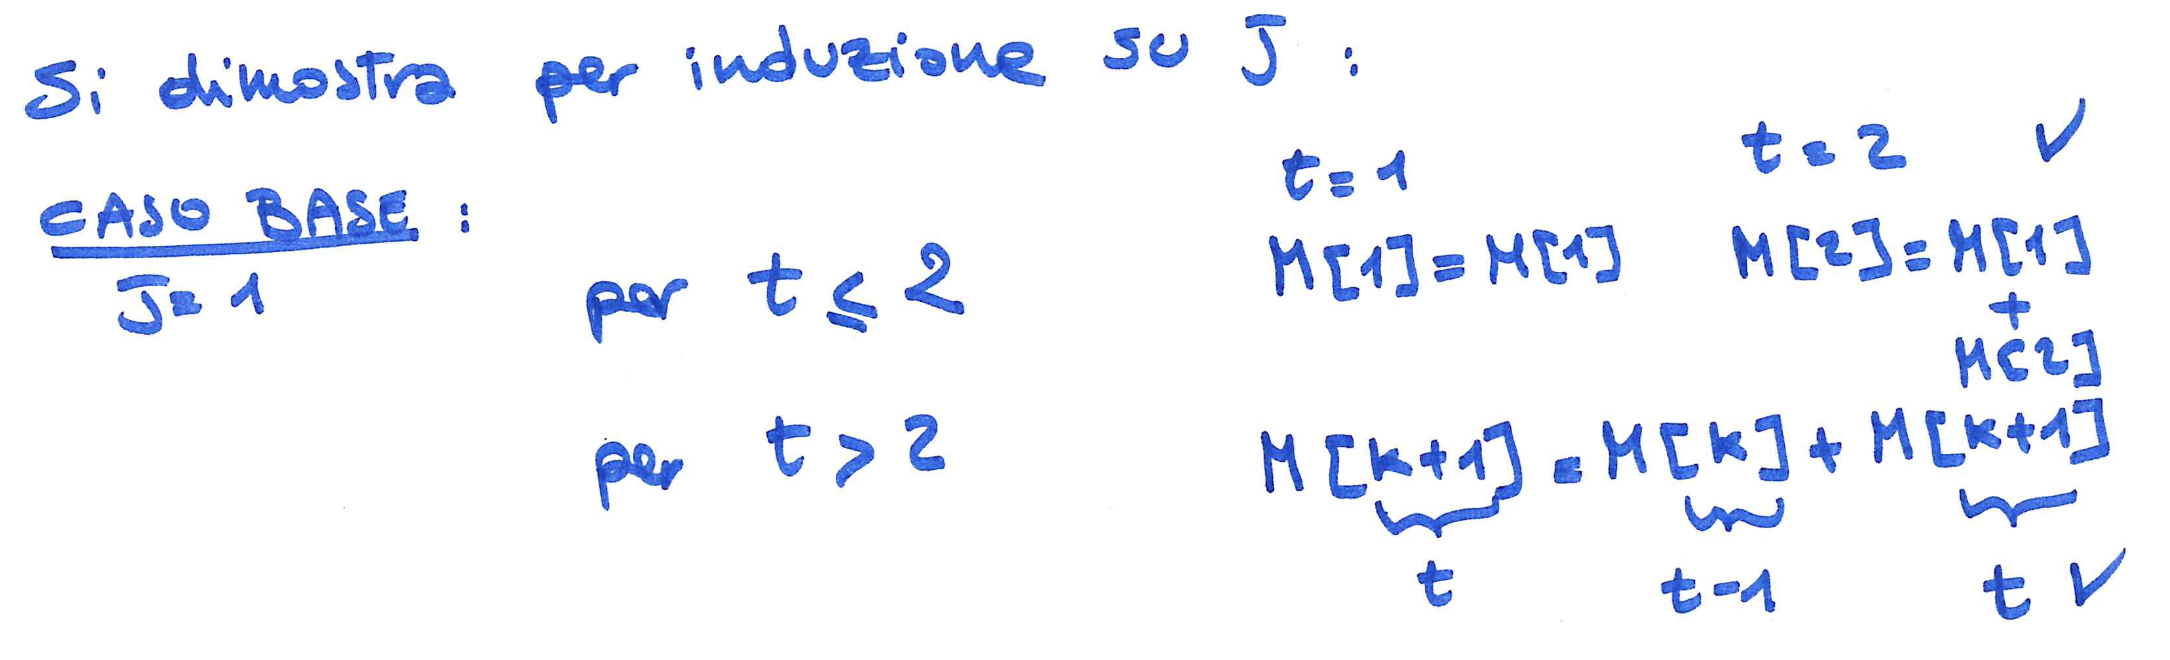
\includegraphics[scale=0.35]{images/dimostrazione_kogge_stone_caso_base.png}
    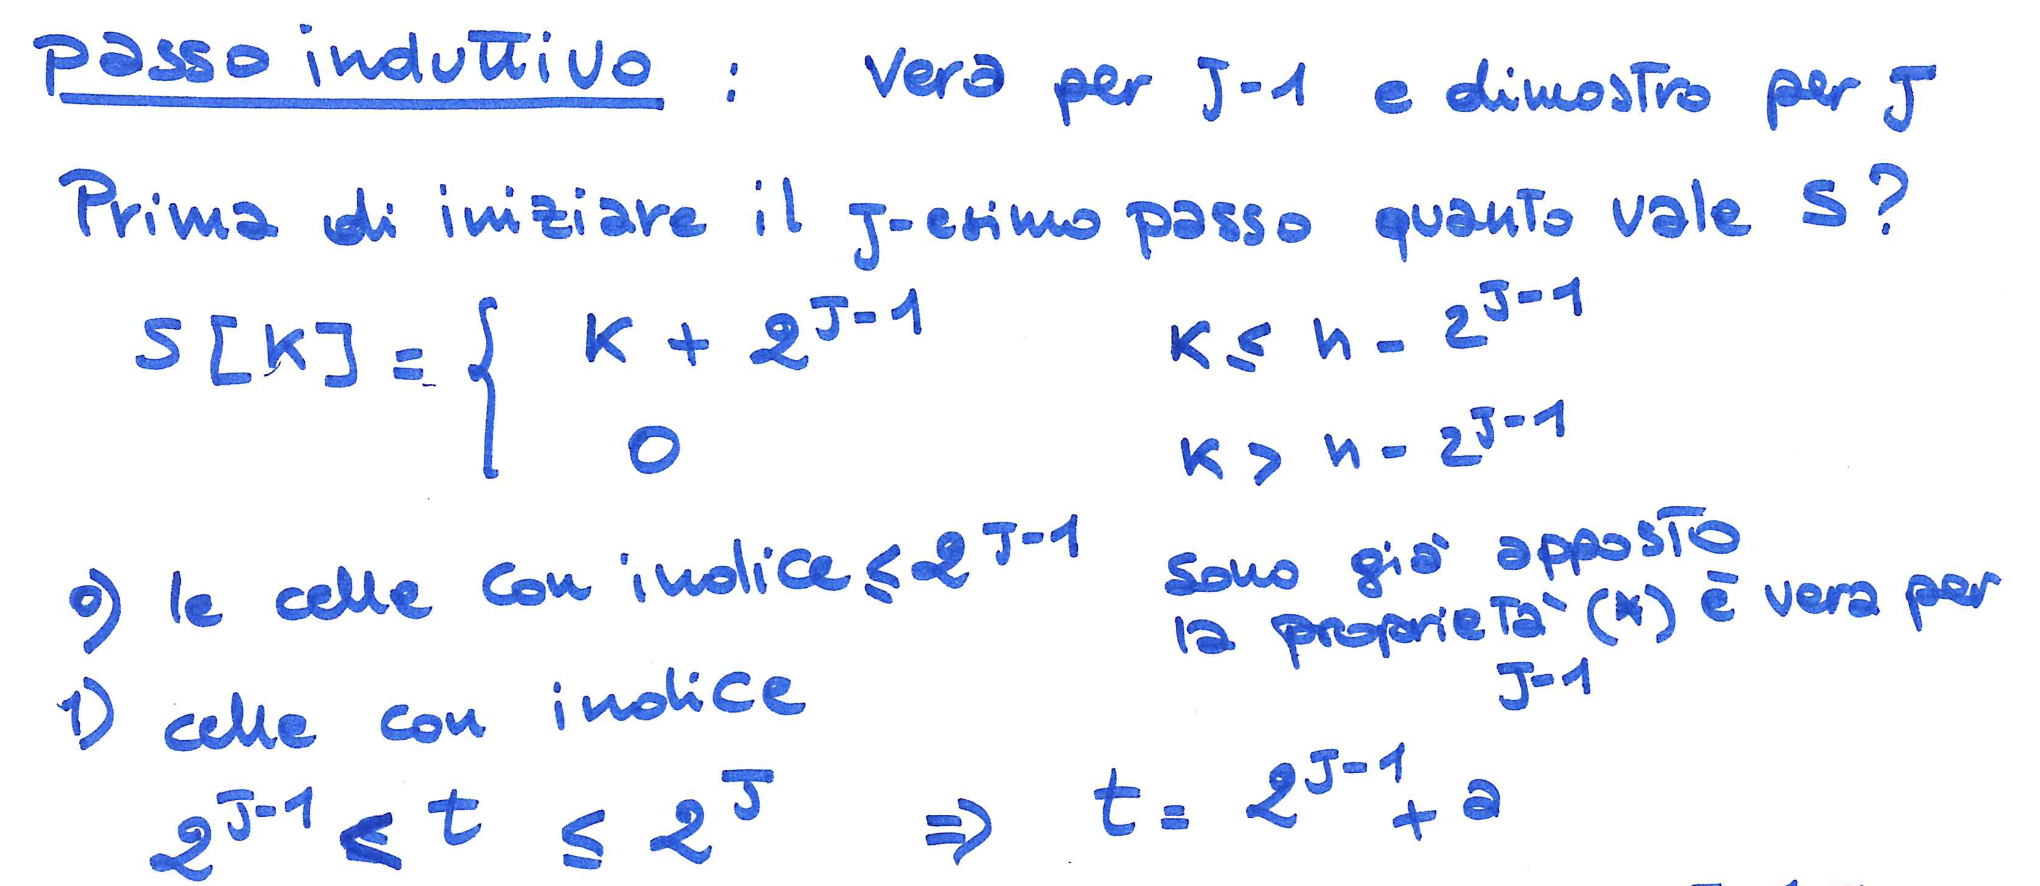
\includegraphics[scale=0.35]{images/dimostrazione_kogge_stone_caso_induttivo.png}
    \caption{Kogge Stone: dimostrazione}
\end{figure}

\begin{figure}[h]
    \centering
    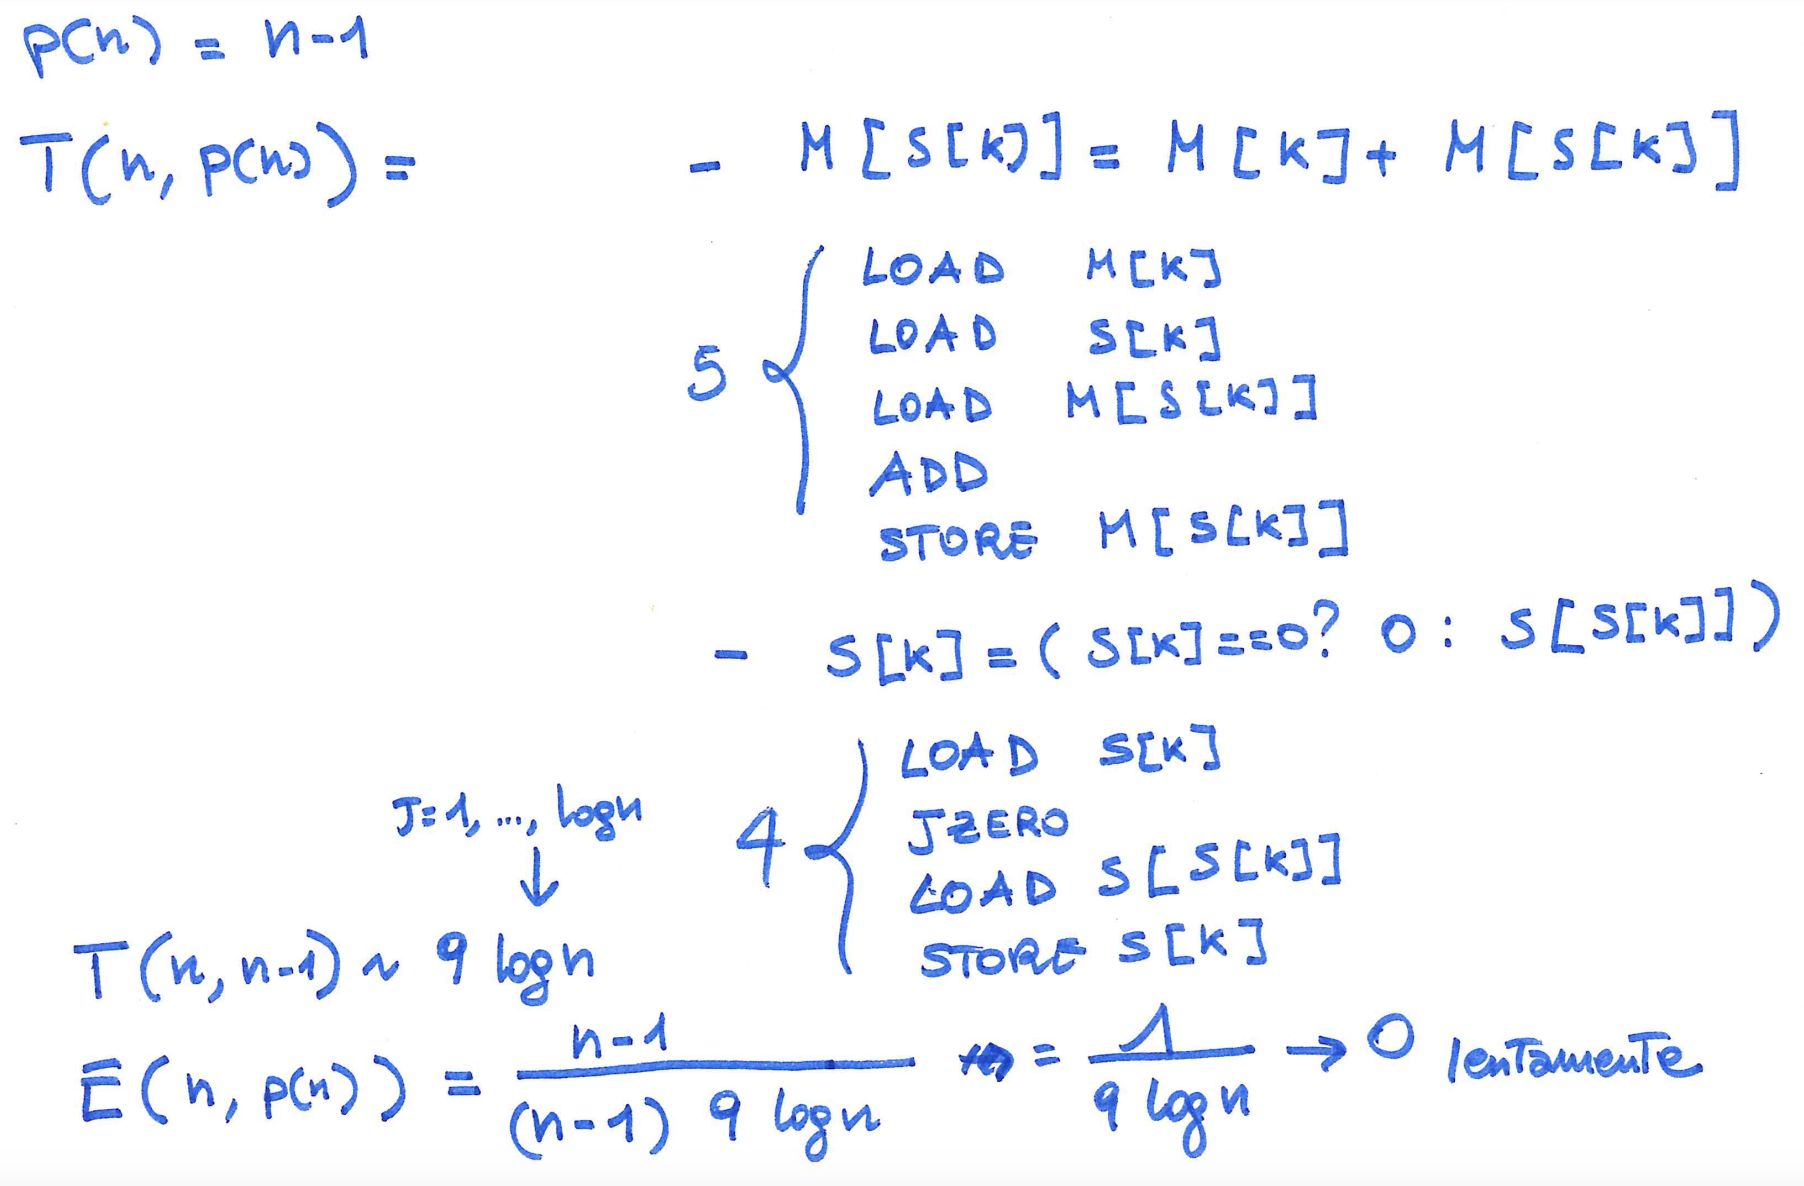
\includegraphics[scale=0.35]{images/valutazione_kogge_stone.png}
    \caption{Valutazione dell'algoritmo Pointer Doubling}
\end{figure}

\paragraph{Sfruttiamo Wyllie come per sommatoria}
Proviamo a raggruppare i processori di $\log n $ in $\log n$ in modo da far sparire la funzione $\log n$ da E
$$p(n) = o(\frac{n}{\log n})\;\;;\; T(n,p(n)) = O(\log n)\;\; ; \; E \rightarrow C \neq 0$$

\begin{comment}
\subsubsection{OP prefissa}
Come per sommatoria anche l'algoritmo dato per somme-prefisse può essere usato per OP-prefissa, dove OP \uline{deve essere associativa}. 

\paragraph{Valutazione dei polinomi}
Sfrutteremo come modulo l'operazione OP-prefissa.

Input: $p(x) = a_0 + a_1x + a_2x^2 + \dots + a_n x^n\; , \; \alpha$\\
Output: $p(\alpha)$

Alle $x$ va sostituito $\alpha$, si eseguono le operazioni sia di potenze che il prodotto con i coefficienti che la somma tra i vari monomi ottenuti.

Dati in memoria condivisa M:
\begin{itemize}
    \item il valore $\alpha$. E' un valore in una cella della memoria
    \item $a_0 + a_1x + \dots + a_n \rightarrow A[0], A[1], \dots , A[n]$. Il polinomio è specificato attraverso i coefficienti $A[i]$ in un vettore della memoria condivisa che chiamiamo $A$
\end{itemize}
Oltre al valore $\alpha$ abbiamo l'input. Le celle dove mettiamo i nostri coefficienti le chiamiamo A.

\paragraph{Algoritmo tradizionale sequenziale}
\begin{itemize}
    \item Numero di prodotti $\appprox n^2$
    \item Numero di somme $n$
\end{itemize}

In buona sostanza, un algoritmo sequenziale efficiente mi richiede $n^2$ operazioni, quindi un tempo quadratico

\paragraph{Miglioramento di Ruffini-Horner (caso sequenziale)}
\uline{Ci porta da un tempo quadratico ad uno lineare, precisamente $2n$}.
L'idea è quella di raccogliere $x$ in maniera iterata

\begin{figure}[h]
    \centering
    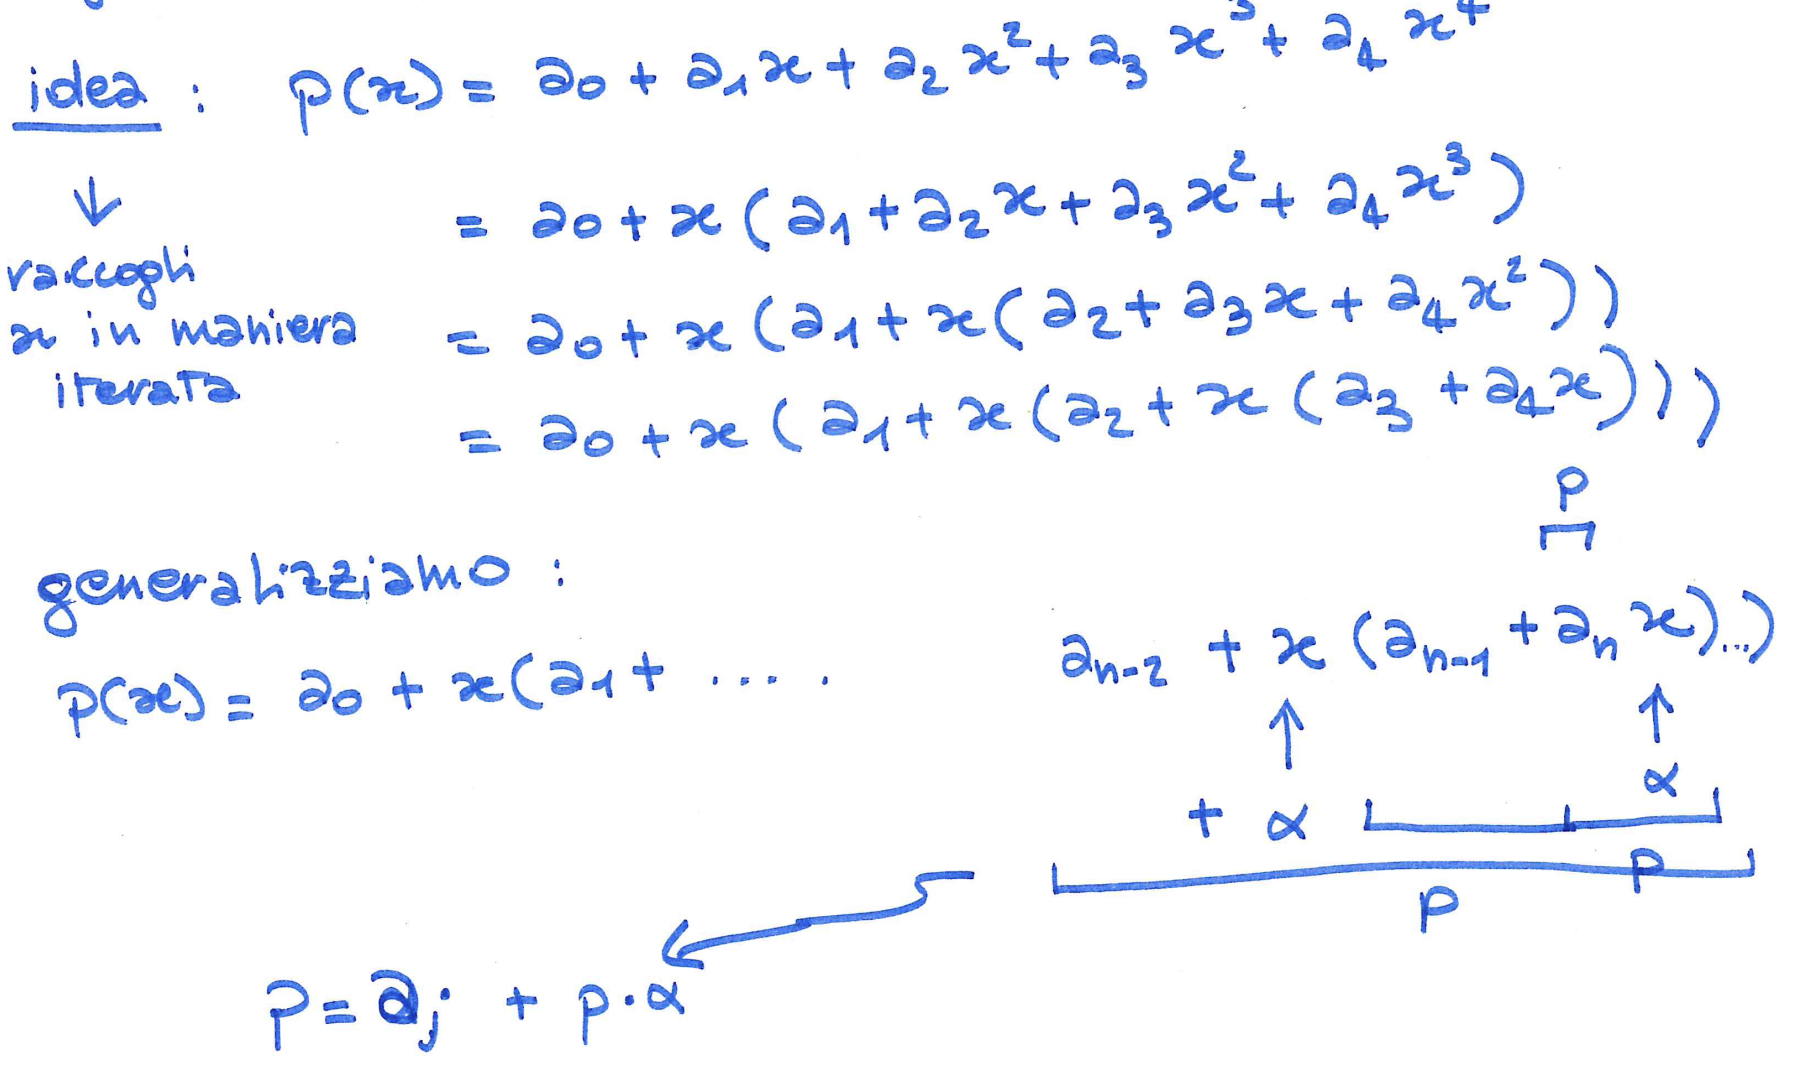
\includegraphics[scale=0.35]{images/ruffini_horner.png}
    \caption{Miglioramento di Ruffini-Horner caso sequenziale}
\end{figure}

Questa nuova forma del polinomio suggerisce un algoritmo, si può prendere una variabile $p$ che è il contenuto delle parentesi tonde. Ogni risultato viene rimesso in $p$

Inizializzo $p = an$, poi $p * \alpha + $ un coefficiente opportuno del mio polinomio e il risultato lo metto in $p$, che a sua volta sarà poi moltiplicato per $\alpha$ e sommato al coefficiente opportuno del polinomio.

L'istruzione $p = a_j + p * \alpha$ è un'istruzione che viene iterata all'interno di un ciclo for che fa variare $j$ opportunamente

\paragraph{Codice per algoritmo sequenziale Ruffini Horner}
\begin{lstlisting}
    Input(alpha)
        p = an
            for i = 1 to n
                p = an-i + p*alpha
    Output(P)
\end{lstlisting}

\paragraph{Prestazioni}
$$T(n,1) = 2n$$
Dobbiamo trovare un algoritmo parallelo che confrontato con questo tempo lineare risulta essere efficiente

\paragraph{Possibile algoritmo parallelo}
\begin{enumerate}
    \item 
    \begin{itemize}
        \item Costruisco il vettore delle potenze di $\alpha\; : \; Q$
        $$Q[K] = \alpha^K\;\;\; 0 \leq K \leq n$$
        E' un vettore nella memoria condivisa dove $$Q[0]=1, Q[1]=\alpha, Q[2]=\alpha^2, Q[n]=\alpha^n$$ 
        \item Eseguo il prodotto interno $<A,Q>$
        $$<A,Q>\;=\sum_{k=0}^n\; A[K]*Q[K]$$
        Quindi valutare i singoli monomi su $\alpha$ e poi sommarli
        \item Restituisco $<A,Q>$, il risultato del prodotto interno 
    \end{itemize}
\end{enumerate}

Per risolvere il punto $(1)$
\begin{itemize}
    \item Metto $\alpha$ in tutti gli elementi di $Q$ da $1$ a $n$
    $$Q[1] = \alpha, Q[2] = \alpha, \dots, Q[n] = \alpha$$
    Non considero la cella $Q[0]$ che deve contenere $1$, poi deve contenere $\alpha$. \uline{Porre tutto ad $\alpha$ significa risolvere un problema che si chiama REPLICA}\footnote{Replicare un valore in ogni elemento di un array}. Se riesco a risolvere il problema replica posso applicare il prodotto prefisso
    \item Applico il PRODOTTO-PREFISSO su $Q$
    $$Q[1] = \alpha, Q[2] = \alpha^2, \dots, Q[n] = \alpha^n$$
    In $Q[2]$ devo fare il prodotto prefisso ed avrò $\alpha^2$, etc. etc, alla fine in $Q[n]$ avrò $\alpha^n$
\end{itemize}

\paragraph{Come risolvere REPLICA in parallelo}

\begin{enumerate}
    \item Utilizziamo una batteria di $n$ processori, ognuno dei quali si occupa di sistemare la cella Q di indice K per K che va da $1$ ad $n$. Quindi ogni processore si occupa di una cella e va ad inserire in questa cella il valore $\alpha$
    \begin{lstlisting}
        for k = 1 to n par do
            Q[K] = alpha;
    \end{lstlisting}
    Questo algoritmo parallelo \uline{non è EREW} perchè abbiamo una lettura simultanea concorrente, se ogni processore si occupa della cella $Q[K]$ e su questo non c'è problema perchè ogni cella è dedicata ad un processore, il problema ce lo abbiamo su $\alpha$. Quando devono caricare $\alpha$ in $Q[K]$ tutti i processori si contendono $\alpha$, avviene una lettura simultanea essendo $\alpha$ in una cella di M condivisa.

    \uline{Questo codice va bene in una architettura CREW}

    Prestazioni di questo algoritmo
    $$p = n \;\; ; \;\; t = 2 \;\; ; \;\; E \approx \frac{n}{n*2} \rightarrow C \neq 0$$
    
    \item 
    \begin{lstlisting}
        for k = 1 to n/logn par do
            for i = 1 to log n do 
                Q[(k - 1) logn + i] = alpha 
    \end{lstlisting}

    Prestazioni di questo algoritmo:
    $$p = \frac{n}{\log n}\;\; ; \;\; t = c \log n \;\; ; \;\; E = \frac{n}{\frac{n}{\log n}\; c \; \log n = \frac{1}{c} \neq 0}$$ 

    Anche in questo caso abbiamo un algortimo CREW, per cui non abbiamo eliminato l'accesso simultaneo ad $\alpha$

    \item Desideriamo un EREW - PRAM, un replica EREW
    \begin{itemize}
        \item costruisci il vettore $\alpha, 0, 0, \dots , 0$ per poi fare che $\alpha$ venga copiato in ognuno di questi zeri. In questo modo avremmo risolto replica. Come è possibile mettere $\alpha$? Passo $2)$
        \item esegui SOMME-PREFISSE
    \end{itemize}

    Questo mi permette di eliminare la lettura concorrente di $\alpha$

    \begin{lstlisting}
        Input(alpha)
        Q[1] = alpha
        for k = 2 to n par do 
            Q[K] = 0
    \end{lstlisting}
    $0$ è una costante che non ha bisogno di essere letta

    
    Ho usato $n$ nel codice ma posso utilizzare \textit{Wyllie} che mi fa passare da $n$ processori a $\frac{n}{\log n}$ processori. Da un tempo costante ad un tempo logaritmico

    Prestazioni di questo algoritmo:
    $$p = \frac{n}{\log n}\;\; ; \;\; t = \log n$$
\end{enumerate}

\begin{figure}[h]
    \centering
    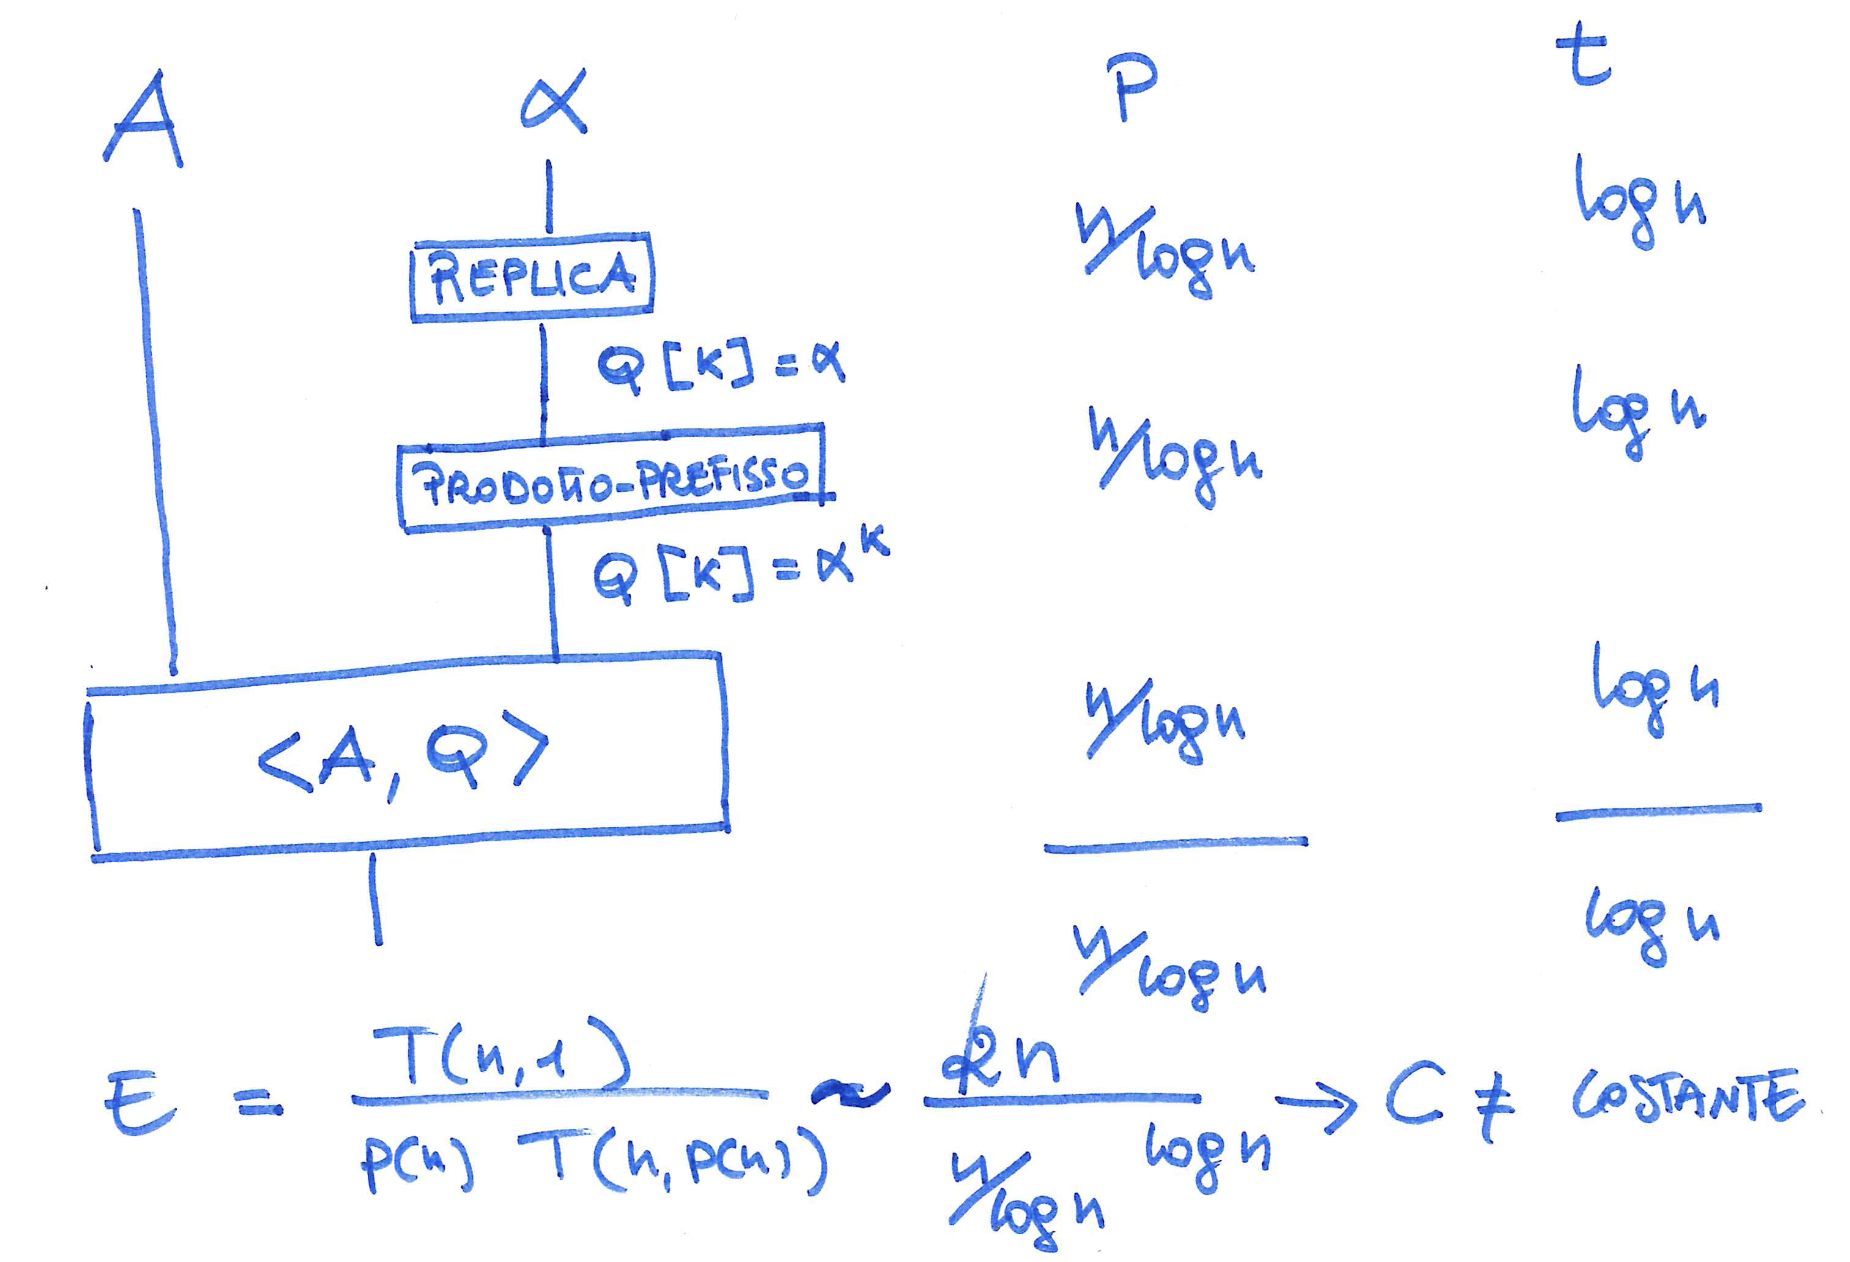
\includegraphics[scale=0.4]{images/valutazione_polinomio_erew_pram.png}
    \caption{Valutazione polinomio EREW PRAM}
    \label{fig:my_label}
\end{figure}
\end{comment}

\newpage


\subsection{Ricerca di un elemento}
Input: $M[1], M[2], \dots , M[n]$\\
Output: $M[n] = 1\; se\; \exists\; k \; t.c. \; M[k] = \alpha$ altrimenti $= 0$

Quando scopro che c'è il valore che sto ricercando vado a posizionare $1$ nella cella $M[n]$. E' una scelta di codice che potrebbe essere infelice se dopo una ricerca ne faccio un'altra.

\paragraph{Algoritmo sequenziale classico}
Richiede $n$ passi, $t = n$. Se l'input è ordinato posso migliorare ad un tempo logaritmico attraverso la ricerca dicotomica.

\paragraph{Algoritmi paralleli per ricerca}
\begin{enumerate}
    \item Proponiamo un algoritmo sull'architettura CRCW. Si utilizzano le celle della memoria M, si usa l'elemento $\alpha$ che è l'elemento da cercare che è input e sta nella memoria condivisa e si utilizza anche un \uline{flag}, anch'esso nella memoria condivisa

    \begin{minted}
    [
    frame=lines,
    framesep=2mm,
    baselinestretch=1.2,
    bgcolor=white,
    fontsize=\footnotesize,
    linenos
    ]{python}
    F = 0
    for k in range(1, n + 1):
        if M[k] == alpha:
            F = 1
    M[n] = F
    \end{minted}

    Se $M[n]$ è uguale a $1$ posso dire di avere trovato $\alpha$ nel mio vettore? Il problema è che non potendo inizializzare $M[n]$ a $0$ (perchè l'n-esimo processore deve accedervi e testare se c'è un valore uguale ad $\alpha$), non posso sapere se $1$ è la soluzione al problema o proprio il contenuto della cella

    Prestazioni di questo algoritmo: $p = n \; , \; t = \text{costante}$

    \item Su architettura CREW, cerca di eliminare la scrittura concorrente. Significa eliminare il flag.

    Trasformiamo il nosto vettore M in un vettore booleano che contiene $1, 0$. Quando una cella contiene $\alpha$ faccio scrivere valore $1$, altrimenti $0$. Dopodichè voglio spostare il risultato nella cella di indice maggiore e posso fare un \textit{MAX-ITERATO} che sposta l'$1$ (se c'è) nell'ultima cella del vettore $M[n]$

    \begin{minted}
    [
    frame=lines,
    framesep=2mm,
    baselinestretch=1.2,
    bgcolor=white,
    fontsize=\footnotesize,
    linenos
    ]{python}
    for k in range(1, n + 1):
        M[k] = 1 if M[k] == alpha else 0
    
    MAX_ITERATO(M[1], ..., M[n])
    \end{minted}

    Prestazioni di questo algoritmo: $p = n \; , \; t = \text{costante}$

    \item Su architetture EREW
    \begin{minted}
    [
    frame=lines,
    framesep=2mm,
    baselinestretch=1.2,
    bgcolor=white,
    fontsize=\footnotesize,
    linenos
    ]{python}
    REPLICA alpha -> A[1], A[2], ..., A[n]
    for k in range(1, n + 1):
        M[k] = 1 if M[k] == A[k] else 0
    
    MAX_ITERATO(M[1], ..., M[n])
    \end{minted}

    Con questo semplice accorgimento della replica abbiamo risolto il problema della concurrent read. Mi ha consentito di passare da un CRCW ad un EREW
    
    Prestazioni di questo algoritmo:\\
    $$p = \frac{n}{\log n}\;\; ; \;\; t = \log n \; \implies E = C \neq 0$$
    
\end{enumerate}

\newpage


\subsection{Ordinamento}
Abbiamo una sequenza di interi e la vogliamo ordinare. Formalmente \textit{RANKING}. 

Input: $M[1], \dots , M[n]$\\
Output: permutazione : $P:{1, \dots, n} \rightarrow {1, \dots , n}$ t.c. $M[P(1)] \leq M[P(2)] \leq \dots \leq M[P(n)]$

dove $p(i)$ è l'indice dell'elemento del vettore M che va in posizione i 

\begin{osservazione}
    In genere gli algoritmi di ordinamento sono basati sui CONFRONTI. Gli algoritmi di ordinamento che usano i confronti hanno un tempo $t = \Theta (n \log n)$. Questo è sia un \textit{upper bound} che un \textit{lower bound}. Upper bound perchè esistono algoritmi come il Merge Sort\footnote{Il Merge sort è un algoritmo di ordinamento che funziona dividendo ricorsivamente una serie di elementi in sottoserie sempre più piccole, fino a quando ogni sottoserie non contiene più di un elemento. A quel punto, le sottoserie vengono ricombinate in ordine crescente, unendo due sottoserie ordinate alla volta, fino a ottenere l'array ordinato finale} che impiega $n \log n$ passi e lower perchè si può dimostrare che se l'algoritmo è basato sui confronti meno di $n \log n$ passi non possiamo fare.
\end{osservazione}

\paragraph{Dimensione di lower bound}
Tutto si basa sull'utilizzo nella dimostrazione di un albero di decisione. \uline{Qualsiasi algoritmo che si basa su confronti durante l'esecuzione produce un albero di decisione, o meglio, un cammino all'interno dell'albero di decisione}. L'albero di decisione è l'algoritmo in sè.

E' un albero binario. \uline{Sui nodi abbiamo i confronti} e ha un figlio sinistro e uno destro. Se al confronto la risposta è positiva si scende verso sinistra, altrimenti a destra.

\uline{Le foglie dell'albero di decisione rappresentano la permutazione dell'input p}. Tale permutazione è conseguenza delle risposte e quindi dei confronti che abbiamo fatto e dimostra come l'input deve essere permutato per ottenerlo ordinato. Cioè ogni foglia individua un cammino, questo cammino sono le sequenze di passi che questo algoritmo mi ha fatto eseguire per poter ordinare il mio array.

\uline{L'altezza dell'albero rappresenta il tempo di esecuzione dell'algoritmo perchè l'altezza di un albero rappresenta il cammino più lungo all'interno del mio albero binario}. Il cammino più lungo equivale al caso peggiore, il massimo numero di passi che devo fare per permutare il mio input

\begin{osservazione}
    Il numero di foglie deve essere almeno $n!$, perchè devono prevedere tutti i possibili ordinamenti di $n$ elementi. Se $t$ è l'altezza il numero massimo di foglie è $2^t$ da cui si ricava che
    $$2^t \geq \#foglie \geq n! \implies t \geq \log n$$
\end{osservazione}

\subsubsection{Counting sort}
Un algoritmo basato sul conteggio e richiede un tempo $t = \Theta(n^2)$

Assumiamo che $n$ sia potenza di $2$ con elementi tutti diversi tra loro.

\uline{Useremo un vettore per salvare le posizioni delle celle ed ottenere l'array ordinato}. Perciò se $M[i]$ va in $k$, metterò in $V[i] = k$. 

$V[i]$ mi dice la posizione finale dell'elemento $i$ del vettore. Questa definizione di $V[i]$ mi da la permutazione inversa che io sto cercando

\paragraph{Counting sort sequenziale}.

\begin{minted}
[
frame=lines,
framesep=2mm,
baselinestretch=1.2,
bgcolor=white,
fontsize=\footnotesize,
linenos
]{python}
for i in range(1, n + 1):
    V[i] = 0

for i in range(1, n + 1):
    for j in range(1, n + 1):
        if M[j] <= M[i]:
            V[i] += 1

F = [0] * (n + 1)
for i in range(1, n + 1):
    F[V[i]] = M[i]

for i in range(1, n + 1):
    M[i] = F[i]
\end{minted}

Se vogliamo restituire il vettore V (la permutazione) l'algoritmo termina al secondo for, se vogliamo invece M ordinato continua

\paragraph{Versione parallela} 
Si cerca di rendere parallelo un algoritmo sequenziale già noto
\begin{enumerate}
    \item Possiamo pensare di prendere un numero di processori $n^2$ per ogni $i, j$ e ogni processore esegue il confronto $M[j] \leq M[i]$. Invece di eseguire la fase 2) (il secondo for) in modo sequenziale, utilizziamo un processore per ogni confronto e mettiamo la risposta in una \uline{matrice booleana} $V[i,j]$
    \begin{lstlisting}
        V[i,j] = (M[j] <= M[i] ? 1:0)
    \end{lstlisting}
    
    Cosa rappresenta la i-esima riga della matrice booleana? Individua gli elementi di $M \leq M[i]$. Contando gli $1$ della riga, so quanti elementi sono $\leq M[i]$ 

    \item \uline{Se per ogni $i$ eseguo la sommatoria parallela della i-esima riga}, ottengo nell'ultima colonna della matrice le posizioni che devono assumere i miei elementi $M[i]$. Sto sommando tutti gli $1$ della riga e li sto mettendo nell'ultimo elemento della prima riga
\end{enumerate}


\paragraph{Codice}.

\begin{minted}
[
frame=lines,
framesep=2mm,
baselinestretch=1.2,
bgcolor=white,
fontsize=\footnotesize,
linenos
]{python}
for i in range(1, n + 1):
    for j in range(1, n + 1):
        V[i,j] = 1 if M[j] <= M[i] else 0

for i in range(1, n + 1):
    SOMMATORIA = sum(V[i, j] for j in range(1, n + 1))

for i in range(1, n + 1):
    M[V[i, n]] = M[i]
\end{minted}

Abbiamo $n^2$ processori e ognuno fa confronti su $j,i$. Siccome questi processori fanno confronti in parallelo gli indici $i,j$ vengono utilizzati $n$ volte. Quindi \uline{la lettura di questi elementi non è esclusiva per processore ma è una lettura simultanea}. \uline{Non possiamo dire che il nostro algoritmo è EREW}.

Per la scrittura diciamo che ogni processore ha la sua cella dove scrive quindi sicuramente non c'è concorrenza sulla scrittura.

\paragraph{Algoritmi di ordinamento paralleli}
\begin{itemize}
    \item Counting-sort 
    $$E = \frac{\log n}{n} \rightarrow 0$$
    \item Bit-sort 
    $$E = \frac{1}{\log n} \rightarrow 0$$
    E' un buon algoritmo parallelo che però non ha ancora un'efficienza costante, ha un'efficienza che tende a zero anche se ci tende lentamente 
\end{itemize}

\subsubsection{Bitonic sort}
Prende spunto dal \textit{Merge sort} ma mette in gioco nuove idee, in particolare nuove sequenze chiamate \uline{unimodali} e \uline{bitoniche}. Il nome deriva appunto da bitoniche, perciò bit-sort (bitonic-sort)

\paragraph{Algoritmo Merge Sort sequenziale}
Utilizza la \uline{tecnica divide et impera}, prende cioè un array di lunghezza $n$ e lo divide richiamando se stesso in due metà. \textit{Merge} fonderà due array già ordinati

\begin{minted}
[
frame=lines,
framesep=2mm,
baselinestretch=1.2,
bgcolor=white,
fontsize=\footnotesize,
linenos
]{python}
if len(A) > 1:
    As = Mergesort(A[0:n//2])
    Ad = Mergesort(A[n//2:])
    A = Merge(As, Ad)
return A
\end{minted} 

Questo \textit{MergeSort} viene chiamato ricorsivamente fino ad ottenere un unico elemento. Nel caso peggiore ogni elemento viene confrontato con due elementi dell'altro array. Perciò $t = n$ nel caso peggiore

Tempo di Merge-sort:\\
\begin{equation}
    t(n) = 
        \begin{cases}
            0 & \text{n=1, ritorna A}\\
            2t(\frac{n}{2})+n  & \text{altrimenti}
        \end{cases}
\end{equation}

\begin{figure}[h]
    \centering
    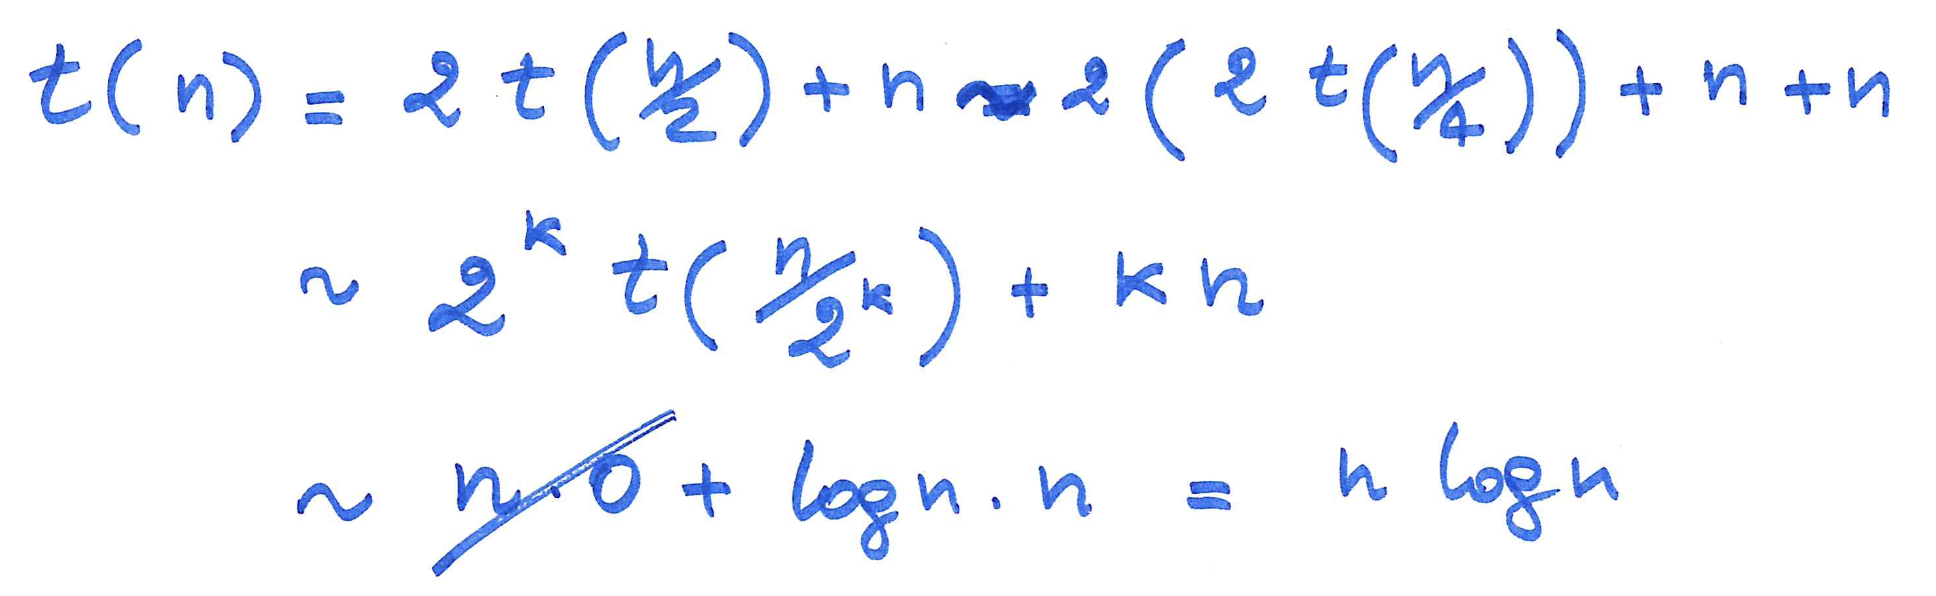
\includegraphics[scale=0.35]{images/merge_sort_tempo.png}
\end{figure}

Se usassi un parallelo quello che mi costa è l'operazione di merge, la divisione dell'input non mi costa niente. Purtroppo il \textit{Merge} non è parallelizzabile, lo devo tenere così com'è e ottengo ancora $T \approx n \log n$

Al posto di chiedersi qual'è il caso peggiore. Quando \textit{Merge} è facile?  

E' facile quando gli elementi di $A_s$ sono tutti minori di $A_d$, in questo caso basta concatenare i due array.
\uline{Dobbiamo cercare di trasformare il nostro input in modo che il Merge faccia questa semplice operazione}

Da qui nasce l'idea per un buon algoritmo parallelo che fa uso di particolari sequenze numeriche che si chiamano \textbf{UNIMODALI} e \textbf{BITONICHE}. Oltre a queste abbiamo bisogno anche di ulteriori routine \uline{REV} e \uline{MIN MAX}. Queste sono funzioni richiamate dal \textit{bit-sort} per cui saranno effettuate in parallelo

\paragraph{Funzione REV}
Fa il reverse di un array. Si leggono i valori $A[1]$ e $A[n]$ e si scambiano di posizione. Si swappano coppie di elementi, che inizialmente sono il primo e l'ultimo e poi si passa al secondo e al penultimo.

Algoritmo parallelo:
\begin{minted}
[
frame=lines,
framesep=2mm,
baselinestretch=1.2,
bgcolor=white,
fontsize=\footnotesize,
linenos
]{python}
for k in range(1, n//2 + 1):
    A[k], A[n - k + 1] = A[n - k + 1], A[k]
\end{minted}

Fa lo swap degli elementi a pari distanza rispetto al centro.

Siccome le coppie sono $\frac{n}{2}$, avrò processori $p = \frac{n}{2}$. Tempo costante

\paragraph{Funzione MIN-MAX}
Permette di costruire gli array $A_{min}$ e $A_{max}$.\\
Considera sempre l'array in due metà, confronta gli elementi a coppie prendendo un elemento della prima metà e uno della seconda metà. In particolare gli elementi devono essere a distanza $\frac{n}{2}$. Da questi confronti vengono fuori il minimo e il massimo. Gli elementi della prima metà $A_{min}$ contengono i minimi, gli elementi della seconda metà $A_{max}$ contengono i massimi

Algoritmo parallelo:
\begin{minted}
[
frame=lines,
framesep=2mm,
baselinestretch=1.2,
bgcolor=white,
fontsize=\footnotesize,
linenos
]{python}
for k in range(1, n//2 + 1):
    if A[k] > A[k + n//2]:
        A[k], A[k + n//2] = A[k + n//2], A[k]
\end{minted}

Anche in questo caso impiego $p = \frac{n}{2}$ processori. Lo SWAP costa $4$, qui c'è un confronto (quindi una micro-istruzione in più). Il tempo è dato da $5$ micro-istruzioni. \uline{Tempo costante}

\paragraph{Particolari sequenze numeriche}
\begin{itemize}
    \item UNIMODALE\\
    Una sequenza è detta unimodale sse $\exists\; k$ che fa da elemento minimo della sequenza per cui da $1$ fino a $k$ i miei elementi decrescono, da $k$ fino ad $A[n]$ i miei elementi crescono. Quindi ho un minimo che è l'elemento $A[K]$.

    Esiste una posizione tale per cui la mia sequenza cresce e poi decresce 
    $$A[1] > A[2] > \dots > A[K] < A[K+1] < \dots$$
    Oppure è vero il viceversa
    $$A[1] < A[2] < \dots > A[K] > A[K+1] > \dots$$
    $A[K]$ invece di essere un minimo è un massimo. Gli elementi decrescono fino ad arrivare a $k$ e poi crescono. \uline{Parzialmente ordinata}
    \item BITONICA\\
    Una sequenza è detta bitonica quando \uline{può essere trasformata in una sequenza unimodale mediante una permutazione ciclica di se stessa}.

    Cioè esiste un $j$ tale per cui prendendo gli elementi da $A[j]$ fino ad $A[n]$ concatenato ad $A[1]$ fino ad $A[j-1]$ ho una sequenza unimodale.

    Ho preso un suffisso della sequenza, l'ho reso un prefisso della sequenza ed ho trasformato in una unimodale, ora esisterà un $k$ che sarà valore minimo o massimo
\end{itemize}

\begin{figure}[h]
    \centering
    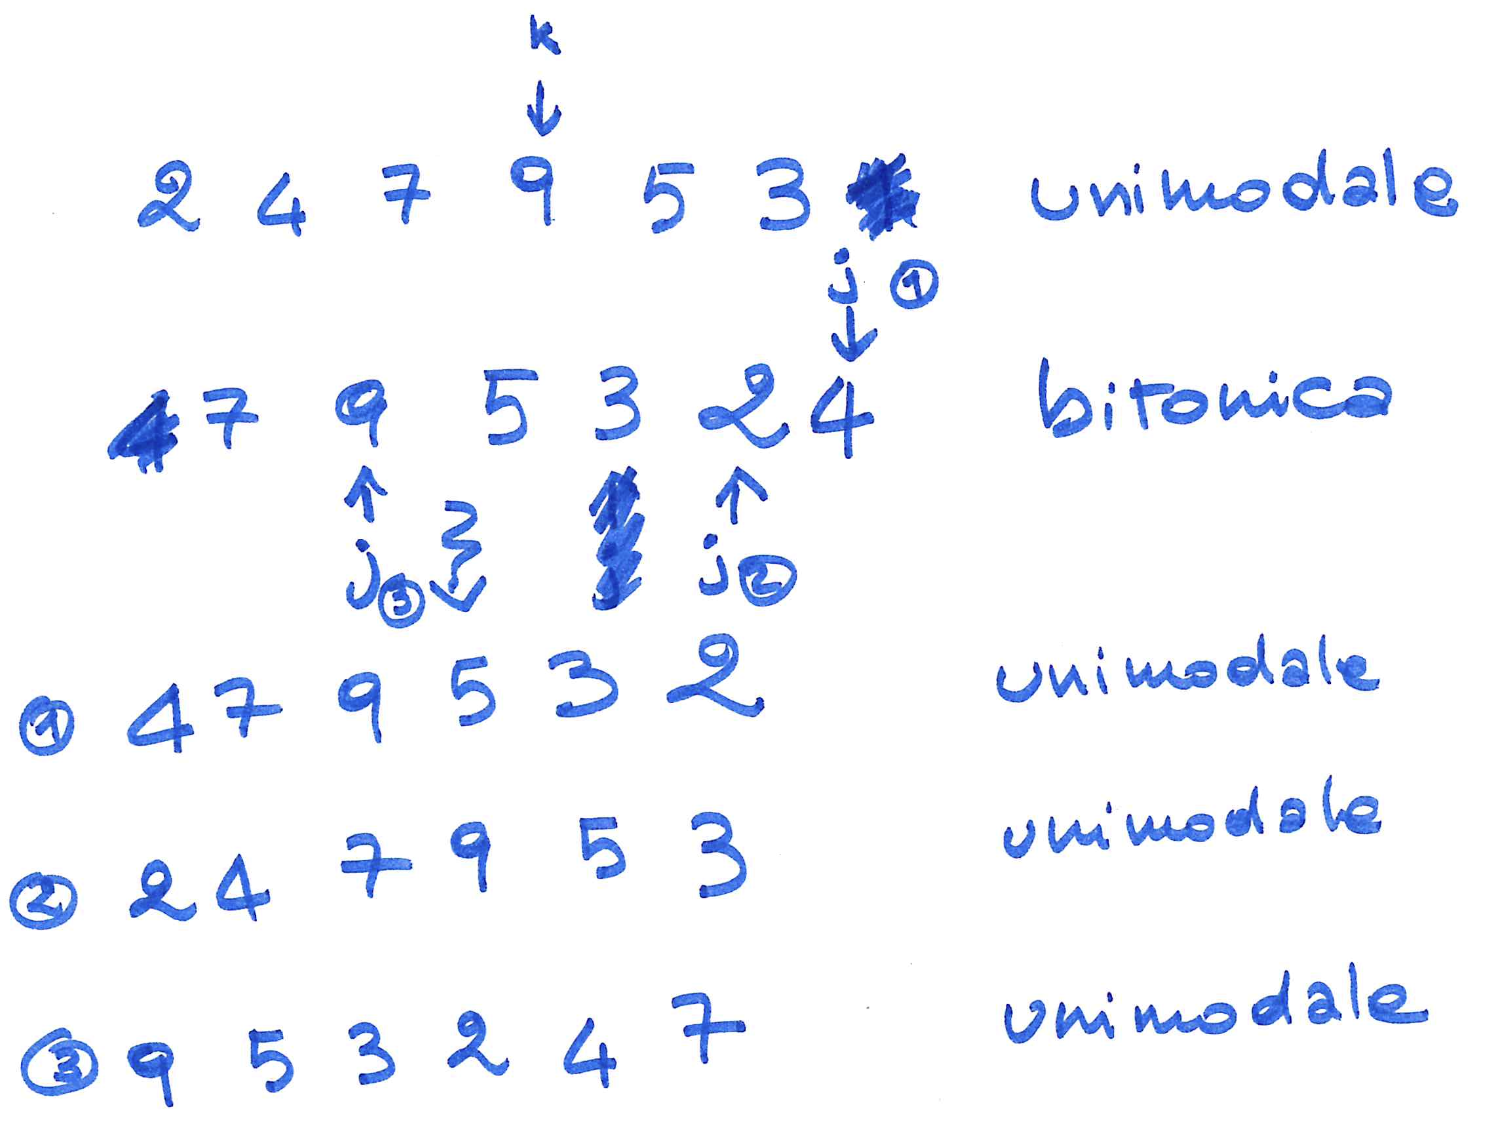
\includegraphics[scale=0.4]{images/bitonica1.png}
\end{figure}

\begin{figure}[h]
    \centering
    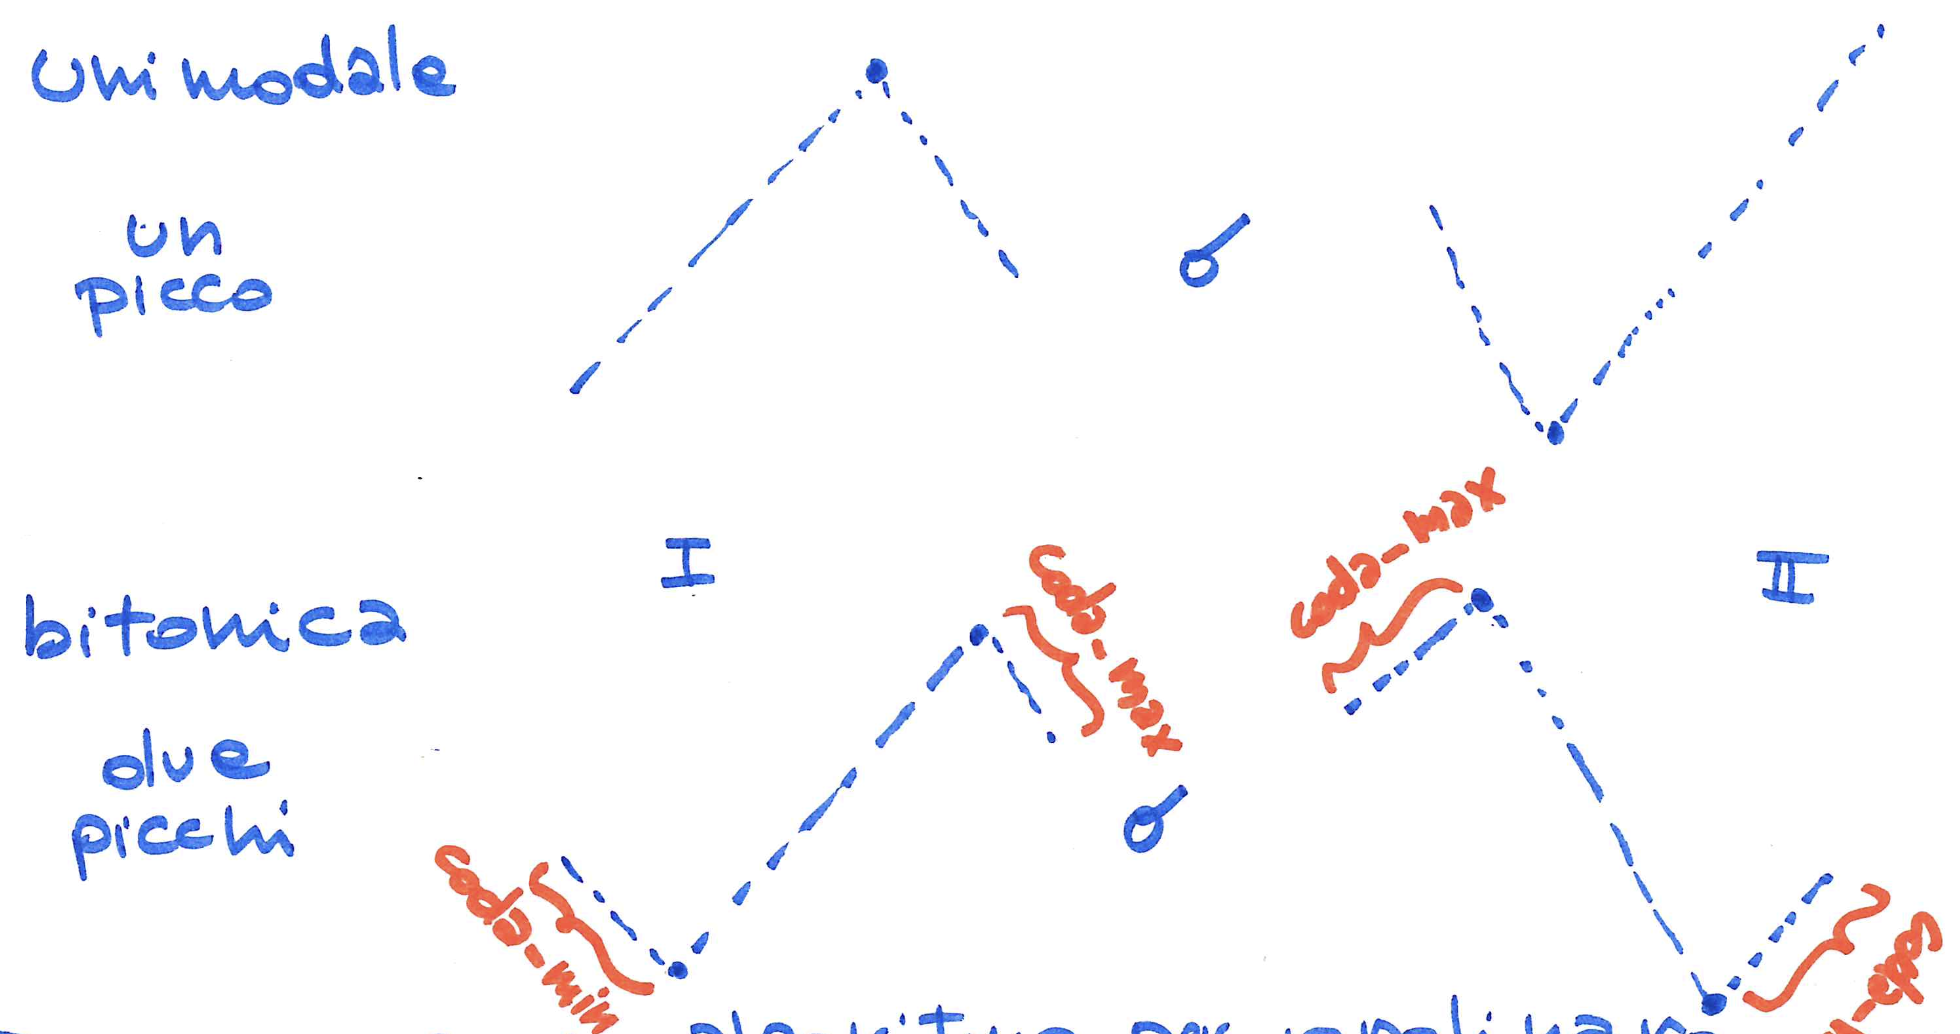
\includegraphics[scale=0.35]{images/bitonica2.png}
\end{figure}


I grafici sono ottenuti plottando gli elementi della sequenza sul piano. Posso spostare \textit{coda-min} e \textit{coda-max} in modo da traformare i due picchi in un picco, traformando così la bitonica in unimodale.

%Bit merge
\subsubsection{Bit merge}
\begin{osservazione}
    Se una sequenza è unimodale è anche bitonica
\end{osservazione}

\begin{osservazione}
    Siano $A, B$ due sequenze ordinate crescenti la sequenza $A * REV(B)$ è unimodale
\end{osservazione}

\paragraph{Proprietà} Se effettuo \textit{MIN-MAX} su una sequenza A
\begin{enumerate}
    \item $A_{min}$ e $A_{max}$ sono ancora bitoniche
    \item $A_{min}$ è fatto di elementi minori degli elementi di $A_{max}$
\end{enumerate}

Tali proprietà suggeriscono un approccio divide-et-impera:
\begin{enumerate}
    \item MIN-MAX suddivide il problema su $n$ elementi in istanze più piccole ($\frac{n}{2}$): $A_{min}$, $A_{max}$  grazie alla proprietà $1$
    \item Ordinando $A_{min}$ e $A_{max}$ la fusione (merge) avviene per concatenazione grazie alla proprietà $2$. Se sono ordinati l'array ordinato si ottiene banalmente concatenando
\end{enumerate}

\paragraph{Algoritmo sequenziale}:
\begin{minted}
[
frame=lines,
framesep=2mm,
baselinestretch=1.2,
bgcolor=white,
fontsize=\footnotesize,
linenos
]{python}
MIN_MAX(A)
if len(A) > 2:
    bit_merge(Amin)
    bit_merge(Amax)
return A
\end{minted}
\textit{bit-merge} ordina le sequenze bitoniche. Restituendo A ritorno due liste ordinate crescenti e concatenandole ottengo il risultato. Correttezza di bit-merge: Si utilizza l'induzione
\begin{itemize}
    \item Caso base: $n=2$\\
    Entro con un input di due elementi, \uline{dopo il MIN-MAX il vettore è ordinato}. Il minimo in prima posizione, il massimo in seconda. Una sequenza di lunghezza $2$ è banalmente ordinata da \textit{MIN-MAX}
    \item Passo induttivo\\
    Supponiamo che per $n = 2^k$ l'algoritmo sia corretto\\
    Dimostriamo che è valido per $A = 2^k + 1$\\
    $A_{min}$ e $A_{max}$ restituiti sono lunghi la metà, quindi $2^k$, vengono passati a \textit{bit-merge}. Abbiamo assunto (ipotesi induttiva) che per quell'ordine di lunghezza l'algoritmo è corretto quindi vengono fuori ordinati e la concatenazione lavora perchè gli elementi di $A_{min} < A_{max}$
\end{itemize}

\paragraph{Implementazione parallela}

%Image lesson 12 parte 2 26.35''

All'inizio c'è un unico \textit{MIN-MAX}, poi viene richiamato da \textit{bit-merge}. All'i-esimo passo mi aspetto i chiamate a \textit{MIN-MAX} su dimensione dell'input $\frac{n}{2^{i-1}}$ fino ad arrivare a \textit{MIN-MAX} effettuato a $2$ elementi, a quel punto si ferma la chiamata ricorsiva

\paragraph{Valutazione}
Lavora su dati diversi di input, perchè ogni volta divide l'input. Ogni \textit{MIN-MAX} lavora su input diversi perciò è EREW P-RAM.

\paragraph{Tempo}
Mi fermo quando $\frac{n}{2^{i-1}} = 2$ da cui ottengo che $i = \log n$. L'albero che disegnamo dove si esegue l'algoritmo parallelo ha profondità logaritmica.

\paragraph{Processori}
Il primo passo parallelo richiede $\frac{n}{2}$ processori. Il secondo passo ne richiede la metà per due $\frac{n}{4} + \frac{n}{4} = \frac{n}{2}$ etc. Quindi ogni passo sostanzialmente richiede $\frac{n}{2}$ processori. 

\paragraph{Efficienza}
$$E = \frac{n \log n}{\frac{n}{2} \; 5 \log n} \rightarrow C \neq 0$$
Sopra il tempo sequenziale di qualsiasi algoritmo che ordina una sequenza numerica. Sotto tempo parallelo. Abbiamo una costante diversa da zero perciò un algoritmo efficiente.


\paragraph{Bit-sort}
Batcher $1968$. Ordina non solo sequenze \textit{unimodali} e \textit{bitonica} e prende spunto dal \textit{bit-merge}

\begin{minted}
[
frame=lines,
framesep=2mm,
baselinestretch=1.2,
bgcolor=white,
fontsize=\footnotesize,
linenos
]{python}
MINMAX(A)
if len(A) > 2:
    bit_sort(Amin)
    bit_sort(Amax)
    bit_merge(Amin * REV(Amax))
return A
\end{minted}

Se entrambi sono ordinati, la fusione la faccio con \textit{bit-merge}, la trasformo in una sequenza unimodale che è anche bitonica. Il bit-merge non faceva la fusione

\paragraph{Correttezza di bit-sort}
Si utilizza l'induzione
\begin{itemize}
    \item Caso base $n=2$\\
    \textit{MIN-MAX} su due elementi li ordina
    \item Passo induttivo\\
    Suppongo che sia corretto per $2^k$ e dimostro che vale per $2^{k+1}$, quindi $|A| = 2^{k+1}$

    \begin{itemize}
        \item \textit{MIN-MAX} divide A in $A_{min}$ e $A_{max}$ di lunghezza $2^k$
        \item bit-sort($A_{min}$) e bit-sort($A_{max}$) li ordinano per ipotesi induttiva
        \item bit-merge($A_{min}\;REV(A_{max})$) ordina A
    \end{itemize}
\end{itemize}

\begin{figure}[h]
    \centering
    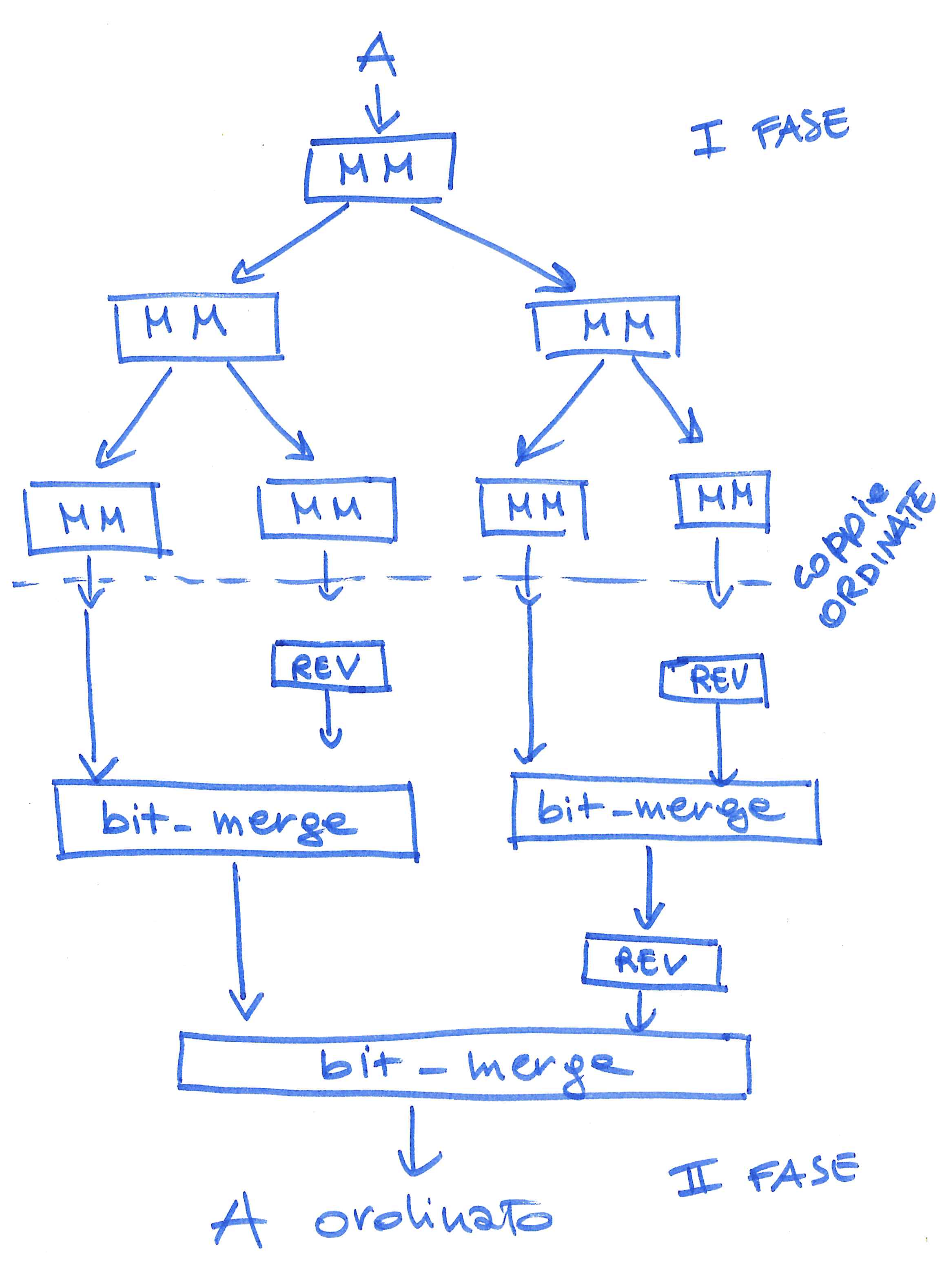
\includegraphics[scale=0.4]{images/bitsort_parallelo.png}
    \caption{Implementazione parallela di bit-sort}
\end{figure}

\paragraph{Valutazione dell'algoritmo}
Questo algoritmo come \textit{bit-merge} è EREW perchè dividiamo ogni volta l'input, non c'è intersezione sui dati su cui lavorano. 

\paragraph{Tempo}
\begin{itemize}
    \item I fase\\
    \textit{i} è l'ultimo passo. (come bit-merge) $i = \log n$. Si esegue MIN-MAX che richiede tempo costante $T(n) = O (\log n)$
    \item II fase\\
    \textit{i} è l'ultimo passo $i = \log n-1$. Si esegue REV costante e bit-merge che richiede $O (\log n) \text{, perciò} \; T(n) = O(\log^2 n)$
\end{itemize}

\paragraph{Processori}
MIN-MAX nella prima fase mi richiede $\frac{n}{2}$ processori, nella seconda fase ho REV e bit-merge, anche loro richiedono $\frac{n}{2}$ processori. Perciò $P = \frac{n}{2}$

%Image lesson 13 parte 1 37.00''

\paragraph{Efficienza}
$$E = \frac{n \log n}{\frac{n}{2}\;5\;\log^2n} \rightarrow \frac{\alpha}{\log n} \rightarrow 0 \;\text{lentamente}$$

\newpage


%Ciclo Euleriano
\subsection{Ciclo Euleriano}
Tecnica applicata in diversi contesti, serve per gestire strutture dati dinamiche. Gestire operazioni su alberi

\paragraph{Definizioni base di Teoria dei Grafi}
\begin{itemize}
    \item Un grafo diretto D è una coppia $(V,E)$ dove $E \in V^2$. Un grafo diretto ha un orientamento. Con la notazione $(\upsilon, \omega)$ denotiamo un arco uscente da $\upsilon$ ed entrante in $\omega$
    \item Cammino: è una sequenza di archi $e_1, e_2, \dots , e_i, e_{i+1}, \dots , e_k$ c'è una proprietà tra due nodi consecutivi tale che il nodo finale (pozzo) di $e_i$ coincide con il nodo iniziale (sorgente) di $e_{i+1} \; \forall i$ 
    \item Ciclo: è un cammino tale che il nodo finale (pozzo) di $e_k$ coincide con il nodo iniziale (sorgente) di $e_1$. Quando un nodo ci fa fare una passeggiata sul grafo ma ci riporta a sè stesso
    \item Ciclo euleriano: abbiamo un ciclo in cui ogni arco del grafo compare una ed una sola volta
    \item Cammino euleriano: cammino in cui (come sopra)
    \item Grafo euleriano: si chiama così se è possibile ottenere un ciclo euleriano, cioè un ciclo che mi fa attraversare ogni suo arco
\end{itemize}

C'è una funzione matematica che mi da la risposta a questo problema $\forall \upsilon \in V$ definiamo: 
$$\rho^-(\upsilon) = | {(\omega, \upsilon) \in E} |$$
grado di entrata di $\upsilon$, tutti gli archi che vedono $\upsilon$ come pozzo e
$$\rho^+(\upsilon) = | {(\upsilon, \omega) \in E} |$$
grado di uscita di $\upsilon$, tutti gli archi che vedono $\upsilon$ come sorgente 

\paragraph{Teorema Eulero 1736}
Un grafo D è Euleriano sse $\forall \upsilon \in V\; : \rho^-(\upsilon) = \rho^+(\upsilon)$

E' sufficiente che il numero di archi in entrata di $\upsilon$ sia uguale al numero di archi in uscita. Basta contarli e se sono diversi non sarà Euleriano

\paragraph{Tecnica del ciclo Euleriano}
Viene usata per costruire algoritmi paralleli efficienti che gestiscono stutture dinamiche come alberi binari. Siccome voglio costruire algoritmi paralleli nella mia memoria condivisa PRAM deve esserci la codifica di un albero binario in termini di tabella

\begin{figure}[h]
    \centering
    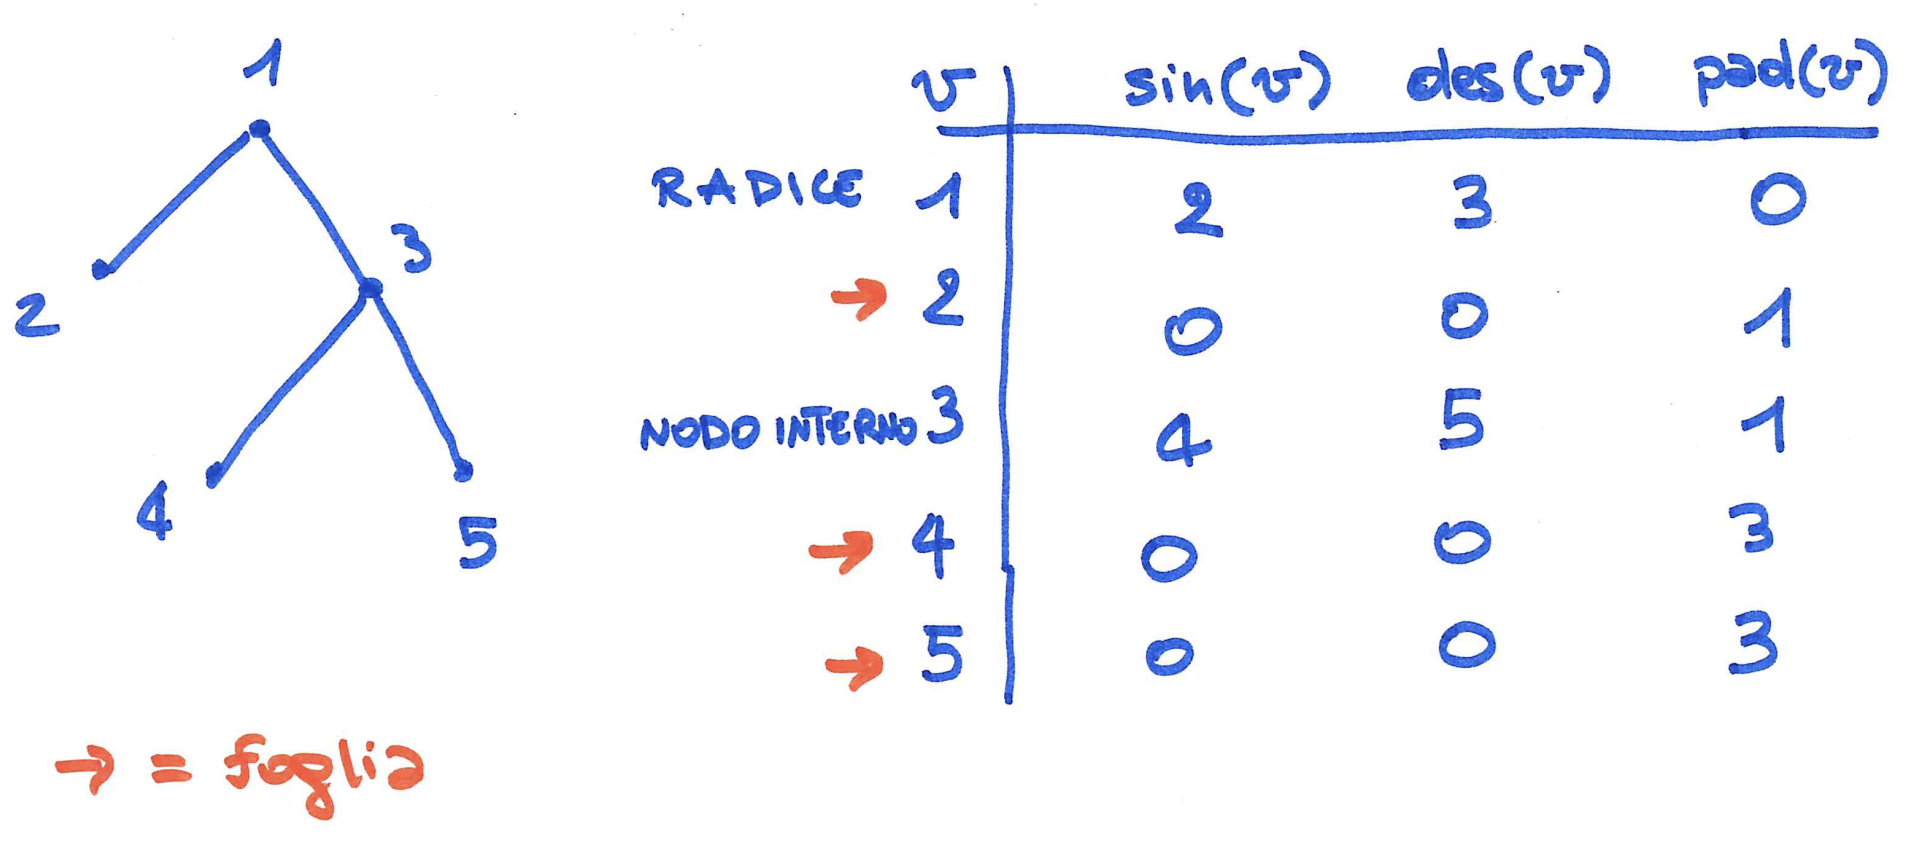
\includegraphics[scale=0.35]{images/ciclo_eureliano.png}
\end{figure}

Come posso rappresentare un albero in una tabella?
\begin{itemize}
    \item Etichetto ogni nodo dell'albero con un numero
    \item Utilizzo una tabella in cui ogni riga è dedicata ad un nodo
    \item Le informazioni che io vado a scrivere su questo nodo (nella colonna) sono: il figlio sinistro ($sin(\upsilon)$), il figlio destro ($des(\upsilon)$) e il padre ($pad(\upsilon)$)
\end{itemize}

Ci dobbiamo immaginare questa tabella in memoria. Molti problemi ben noti usano la struttura dati ad albero: ricerca, dizionari, query. L'operazione fondamentale in questi problemi è la navigazione dell'albero, anche per la manutenzione (inserimento, modifica e cancellazione) di elementi.

Come farlo con algoritmi paralleli efficienti? Usiamo le liste che si gestiscono bene in parallelo (vedi Kogge-Stone). Le liste che non sono altro che dei puntatori ai nodi dell'albero. Dobbiamo sostanzialmente definire un vettore $\vec{s}$ dei successori dell'albero. E' un vettore che lega gli elementi in un array e indica chi è il successore per ogni elemento.

\begin{enumerate}
    \item Dall'albero binario al ciclo Euleriano.\\
    Associo all'albero binario un ciclo Eureliano. Sostituisco ogni ramo dell'albero con due archi, uno che scende e uno che sale.

    \begin{figure}[h]
        \centering
        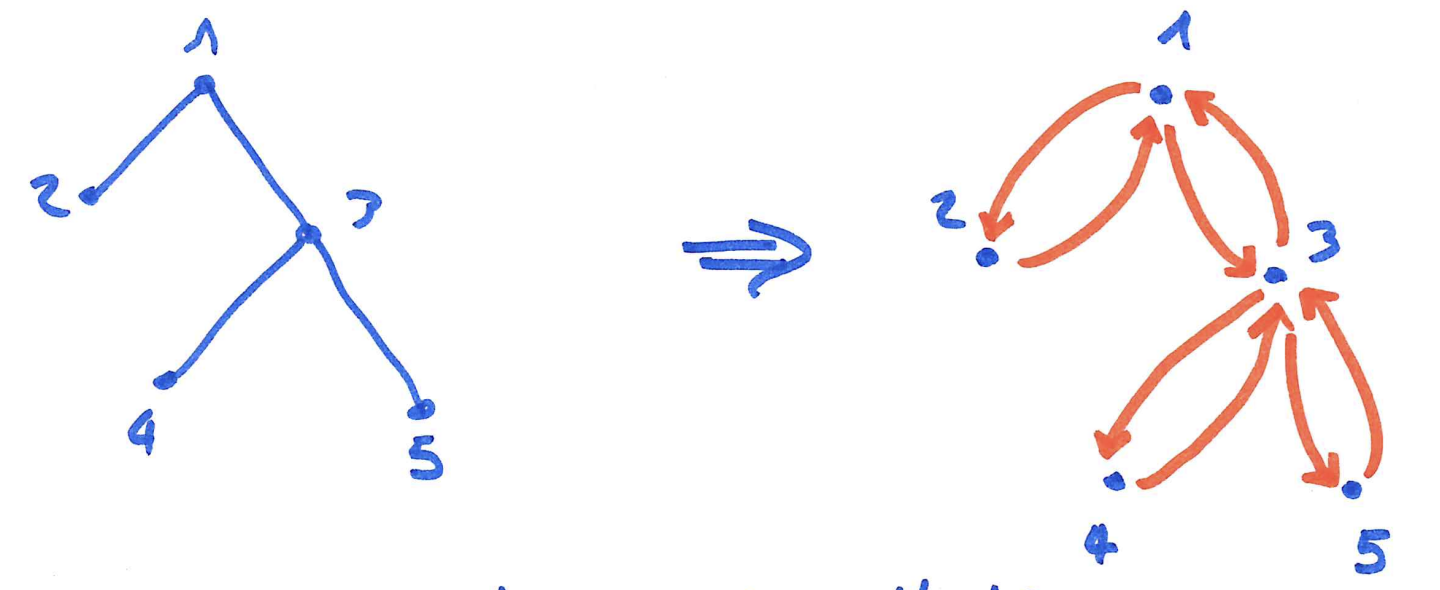
\includegraphics[scale=0.35]{images/ciclo_euleriano1.png}
        \caption{Ciclo euleriano: primo passo}
        \label{fig:my_label}
    \end{figure}

    \item Dal ciclo Eureliano al cammino Eureliano.\\
    Siccome in qualche nodo ci potrebbe essere ambiguità (potrei scendere o anche risalire), trasformo questo grafo in un altro grafo in modo da definire un cammino Eureliano, seguendo questa regola: ogni nodo $\upsilon$ viene espanso in $3$ nodi $(\upsilon, s), (\upsilon, c), (\upsilon, d)$. Rispettivamente sinistra, centro, destra.\footnote{Nonostante sia definita un'etichetta questi non sono da considerarsi degli archi ma sono da considerare come nodi}

    \begin{figure}[h]
        \centering
        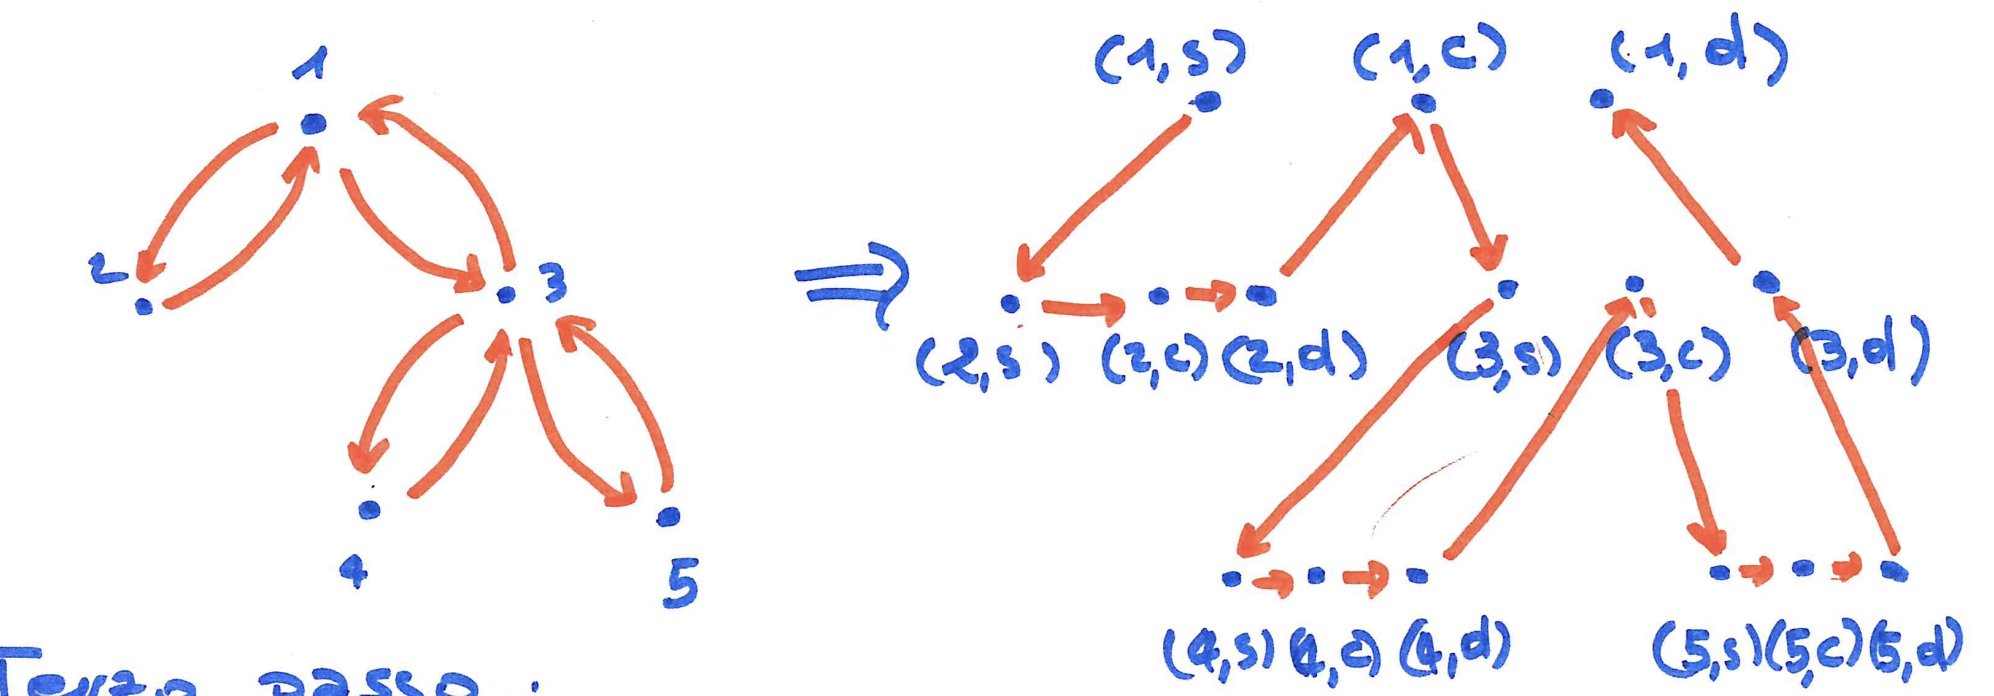
\includegraphics[scale=0.35]{images/cliclo_eureliano2.png}
        \caption{Dal ciclo al cammino Eureliano}
        \label{fig:my_label}
    \end{figure}

    Inserisco delle freccie che collegano tutti i nodi (anche quelli espansi), il cammino che esce fuori è un cammino Eureliano. Questo perchè percorro gli archi una ed una sola volta.

    \item Dal cammino Eureliano alla costruzione della lista.\\
    \uline{Sarà un vettore indicizzato dai nodi del grafo}

    $$S( (\upsilon, x) )\; dove\; 1\leq \upsilon \leq n \; , x \in \{s,c,d\} $$

    \item Costruzione dell'array\\
    Abbiamo delle regole diverse in base a se il nodo è un nodo foglia o un nodo interno 

    Se il nodo foglia è figlio sinistro punta al centro, se figlio di destra punta al nodo padre con etichetta destra

    Se il nodo è interno, se ha un'etichetta sinistra scende al figlio di sinistra con etichetta $s$, se centro scende al figlio di destra con etichetta $s$. Quando è destro vale la stessa regola per il nodo foglia destro

    Diamo un algoritmo parallelo per costruire S. \uline{Trasforma il grafo in una lista dicendo per ogni nodo chi è il successore}. Si può pensare che la tabella è in memoria ed ogni processore prende in carico una riga della tabella (quindi di un vertice) e per ogni riga della tabella costruisce il successore

    Si può eliminare la concorrenza delle letture.
\end{enumerate}

\paragraph{Valutazione}
    Questo algoritmo (con alcuni accorgimenti per eliminare la concorrenza delle letture) risulta essere un EREW 

\paragraph{Processori}  Prima $P = n$; Dopo Willye $P = \frac{n}{\log n}$

\paragraph{Tempo} $T(n, p(n)) = O(1)$\\
Numero di processori $n$, tempo costante è uno di quei casi che ci ricorda che se raggruppiamo con $\log n$ i nostri nodi $\upsilon$ possiamo passare da $n$ a $\log n$ processori e il tempo da costante diventa logaritmico $T = \log n$

\newpage
